\section{Specific Requirements}

\subsection{External Interface Requirements}

\subsubsection{User Interfaces}
The following figures show a mock-up user interface of the mobile application for the Best Bike Paths system. The images exhibit the most important screens from the perspective of a registered user. The home screen shown in figure \ref{fig:home_screens} and the profile screen shown in figure \ref{fig:profile_screen}, are replaced by a direct link to the registration page if the user did access the application without signing up.

\paragraph{Sign In and Sign Up Pages}
In this screen the user can sign in by entering e-mail and password, if already registered. If the user is new to the platform, can click the "\textit{New to the community?}" button and access the sign up screen, where he can enter his name, surname, email and password to create an account. If a registered user accidentally entered the sign up screen, can go back to the sign in screen by clicking the "\textit{Already part of the community}" button. In both screens, non-registered users can access the map screen shown in figure \ref{fig:map_screens} by clicking the "\textit{Let's explore without account}" button. 

\begin{figure}[H]
    \centering
    \begin{subfigure}[b]{0.49\textwidth}
        \centering
        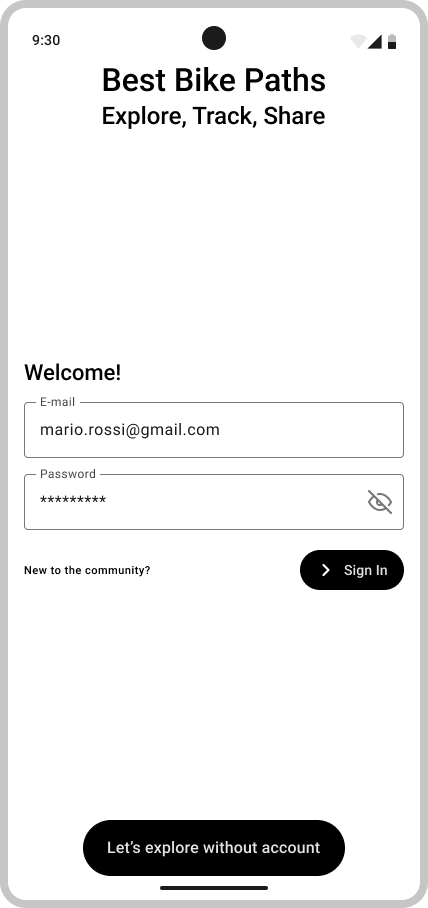
\includegraphics[width=0.5\textwidth]{RASD/source/images/UI/SignIn Screen.png}
        \caption{Sign In Screen.}
        \label{fig:sign_in_screen}
    \end{subfigure}
    \hfill
    \begin{subfigure}[b]{0.49\textwidth}
        \centering
        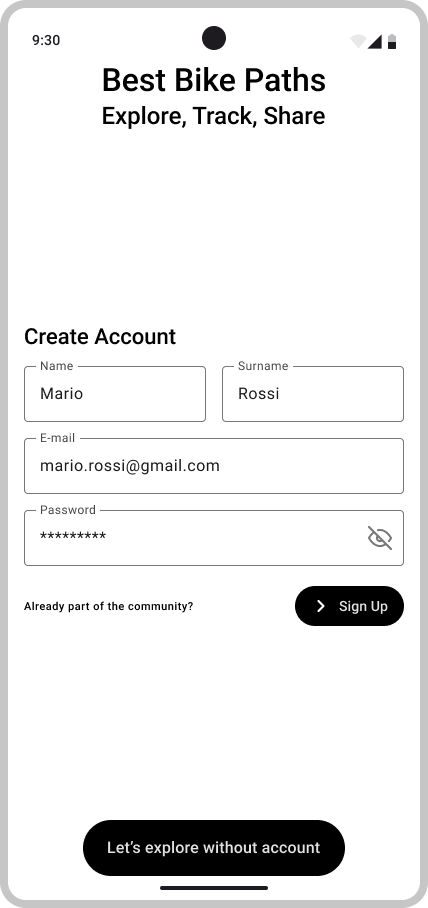
\includegraphics[width=0.5\textwidth]{RASD/source/images/UI/SignUp Screen.png}
        \caption{Sign Up Screen.}
        \label{fig:sign_up_screen}        
    \end{subfigure}
    \caption{Sign in and Sign up screens.}
    \label{fig:sign_in_up_screens}
\end{figure}

\paragraph{Home Screen}
In this screen the registered user can visualize his statistics, the trips he planned and all his biking activities. By clicking on a saved trip, the user can immediately start the navigation of the selected trip, as shown in figure \ref{fig:map_navigation}. By clicking on an activity, the user can see the details regarding that specific activity, like total distance, average speed, total time, elevation and weather conditions, and also the report of all obstacles encountered during his trip. In this screen the user can also delete the activity by clicking on the trash button (top right corner), after confirmation, or go back to the home page by clicking the back button (top left corner). This screen is reserved to \underline{registered users only}.

\begin{figure}[H]
    \centering
    \begin{subfigure}[b]{0.3\textwidth}
        \centering
        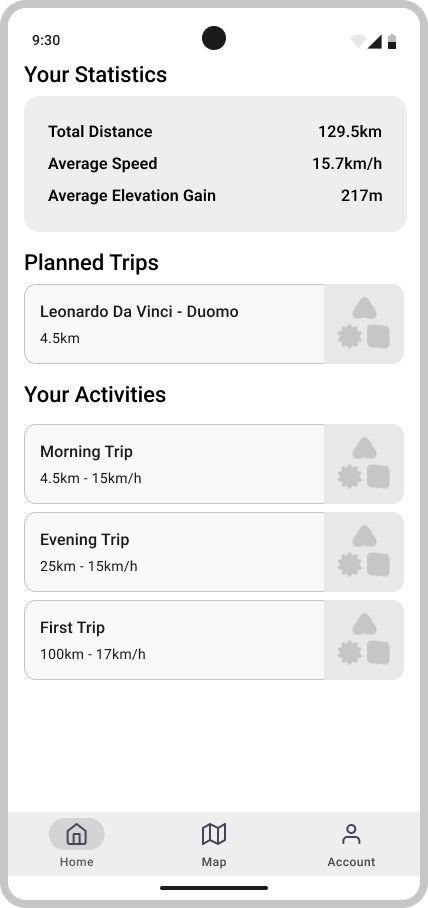
\includegraphics[width=0.75\textwidth]{RASD/source/images/UI/Home Screen.png}
        \caption{Home Screen.}
        \label{fig:home_screen}
    \end{subfigure}
    \hfill
    \begin{subfigure}[b]{0.3\textwidth}
        \centering
        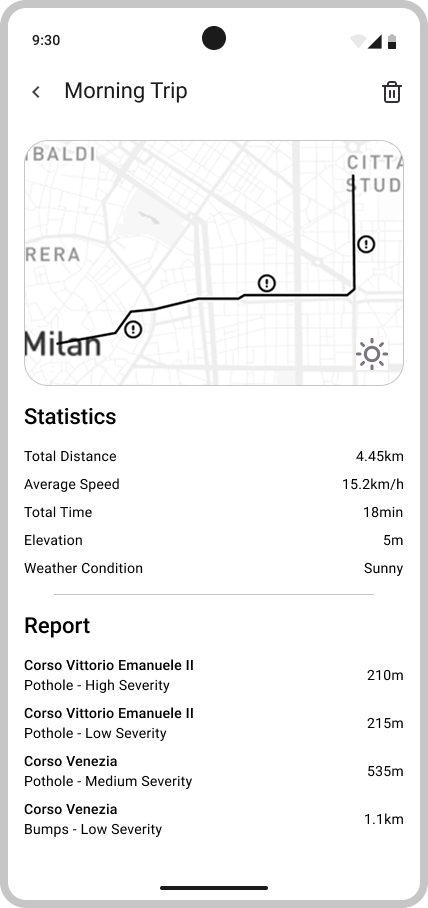
\includegraphics[width=0.75\textwidth]{RASD/source/images/UI/Trip Details Screen.png}
        \caption{Sign Up Screen.}
        \label{fig:detail_screen}        
    \end{subfigure}
    \hfill
    \begin{subfigure}[b]{0.3\textwidth}
        \centering
        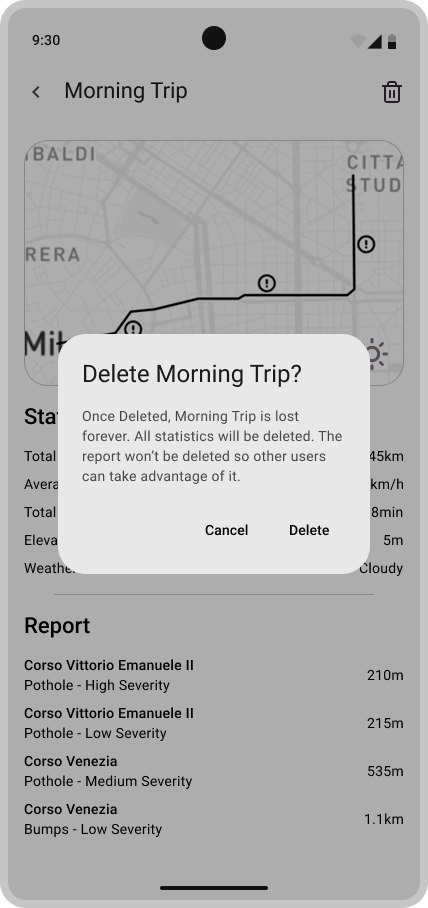
\includegraphics[width=0.75\textwidth]{RASD/source/images/UI/Trip Details Screen - Deletion.png}
        \caption{Deletion of an activity.}
        \label{fig:detail_screen_deletion}        
    \end{subfigure}
    \caption{Home Screen and Trip Details Screen.}
    \label{fig:home_screens}
\end{figure}

\paragraph{Map Screen}
In this screen users can browse the map, visualize their current position on the map, by clicking the first button of the floating menu on the bottom left corner, and change the map orientation by clicking to the second button of the floating menu. By inserting a departure and destination point in the first and second input fields respectively, the user can see on the map different paths that lead from the departure point to the destination one. By clicking on a path, the user can see the major obstacles along the way signalled by other users and the score of every segment of the path coded in different colours. 

The following is reserved to \underline{registered users only}.
When clicking on a path, a switch appears under the input fields, allowing the user to activate automatic data acquisition when cycling. Also a floating action button on the bottom right corner appears, so the user can start biking the selected route. Once clicked, the floating action button reveals two options: "\textit{Save Trip}" or "\textit{Start Trip}", which let the user choose between saving the trip for later cycling sessions, or immediately starting the trip. By pressing the "\textit{Save Trip}" button, the user can visualize his trip in the home screen, shown in figure \ref{fig:home_screen}. By pressing the "\textit{Start Trip}", the user is taken to the navigation page, where he can stop the recording at any time by clicking on the "\textit{Stop Recording}" button, add a new obstacle on his way by clicking the bottom right floating action button with the plus sign. or switch between manual or automatic mode, by clicking the switch in the bottom left corner.

\begin{figure}[H]
    \centering
    \begin{subfigure}[b]{0.49\textwidth}
        \centering
        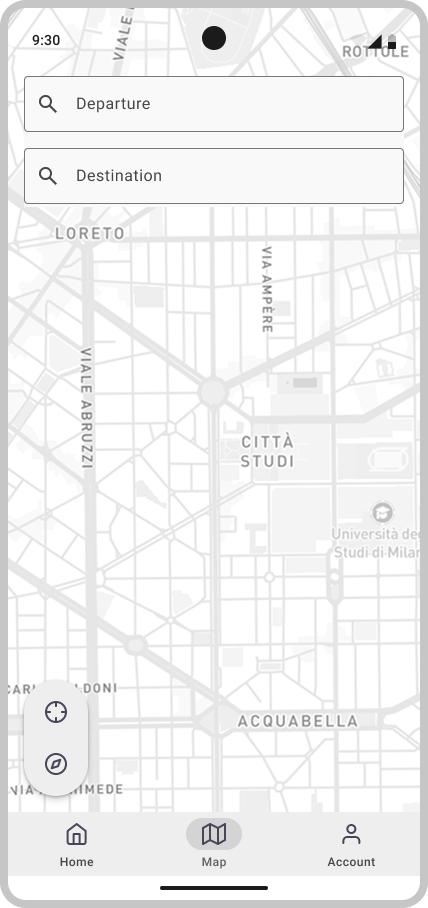
\includegraphics[width=0.5\textwidth]{RASD/source/images/UI/Map Screen.png}
        \caption{Map Screen.}
        \label{fig:map_screen}
    \end{subfigure}
    \hfill
    \begin{subfigure}[b]{0.49\textwidth}
        \centering
        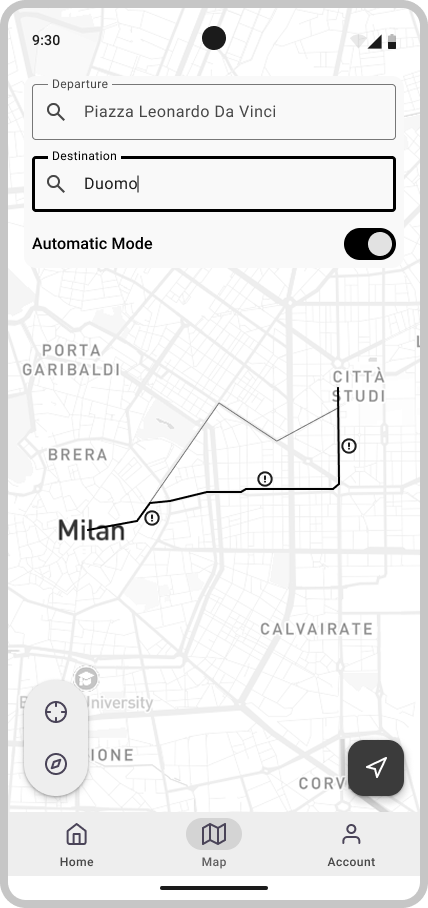
\includegraphics[width=0.5\textwidth]{RASD/source/images/UI/Map Screen - Trip Planning 1.png}
        \caption{Map Screen Trip Planning.}
        \label{fig:map_screen_planning_1}        
    \end{subfigure}
    \hfill
    \begin{subfigure}[b]{0.49\textwidth}
        \centering
        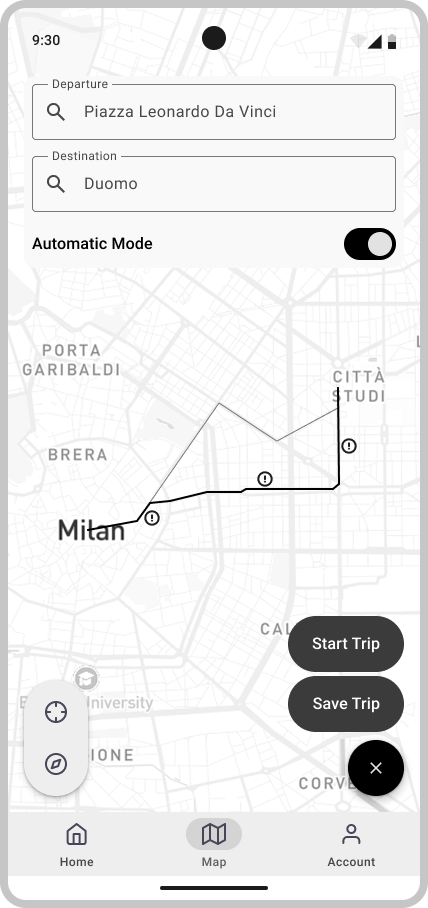
\includegraphics[width=0.5\textwidth]{RASD/source/images/UI/Map Screen - Trip Planning 2.png}
        \caption{Map Screen Trip Selection.}
        \label{fig:map_screen_planning_2}        
    \end{subfigure}
    \hfill
    \begin{subfigure}[b]{0.49\textwidth}
        \centering
        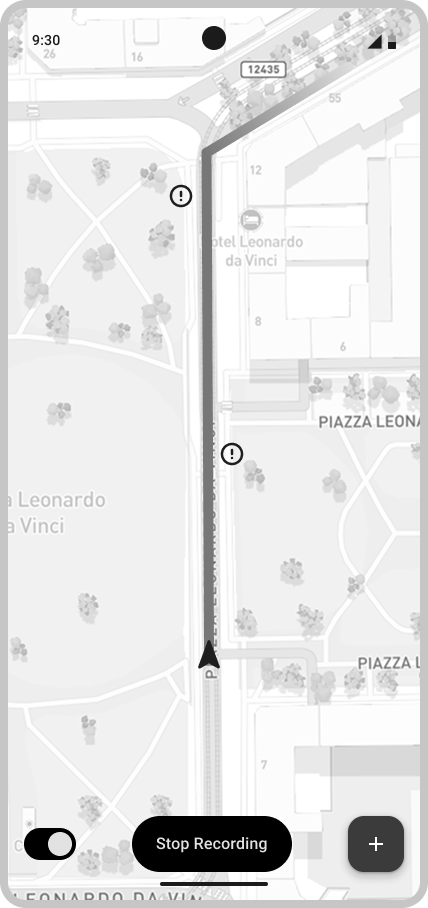
\includegraphics[width=0.5\textwidth]{RASD/source/images/UI/Navigation.png}
        \caption{Map Navigation.}
        \label{fig:map_navigation}        
    \end{subfigure}
    \caption{Map Screens and Navigation.}
    \label{fig:map_screens}
\end{figure}

\paragraph{Report Screen}
This screen is presented to registered users who terminated their biking session. Here can manually add obstacles found along the way, or review the ones added with the floating action button with the plus sign in the bottom right corner found in the previous screen, shown in figure \ref{fig:map_navigation}. Here can manually modify the name of the obstacle, the street where the obstacle was found and the severity of the obstacle. Also, the registered user is suggested with obstacles signalled by other members of the community, so it's easier for him to insert obstacles. The user can also delete obstacles he accidentally inserted, by clicking in the trash icon button next to the name of the obstacle. The same set of operations can be performed by a registered user who chose to automatically gather information when presented with the floating action button option in screen \ref{fig:map_screen_planning_2}. This screen is presented to the user for every street he went through during his journey. He can go the next route by pressing the "\textit{Next}" button or go to the previous one by clicking on the "\textit{Previous}" button. Once the review of the report is completed, the user is presented with a greeting screen, where he can visualize his statistics and go to the home screen. This screen is reserved to \underline{registered users only}.

\begin{figure}[H]
    \centering
    \begin{subfigure}[b]{0.3\textwidth}
        \centering
        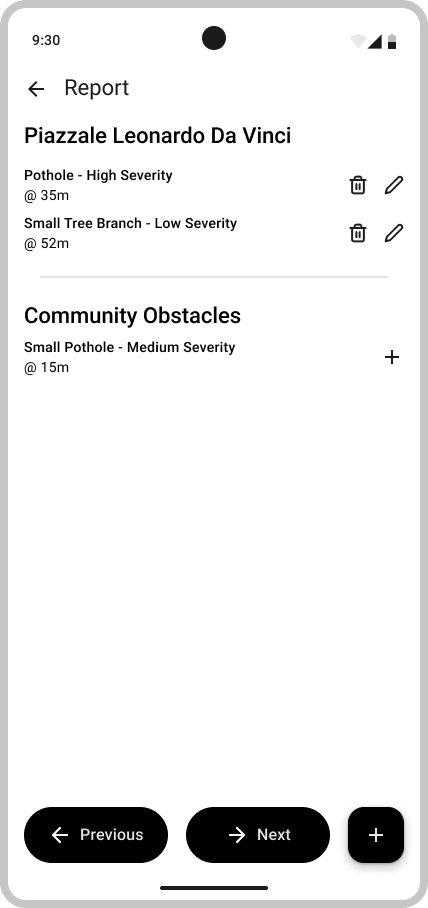
\includegraphics[width=0.75\textwidth]{RASD/source/images/UI/Report Screen.png}
        \caption{Report Screen.}
        \label{fig:report_screen}
    \end{subfigure}
    \hfill
    \begin{subfigure}[b]{0.3\textwidth}
        \centering
        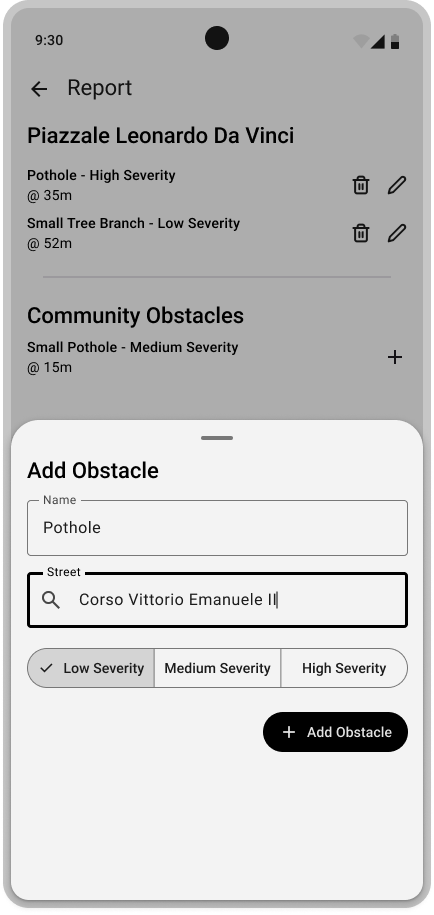
\includegraphics[width=0.75\textwidth]{RASD/source/images/UI/Report Screen - Add obstacle.png}
        \caption{Add obstacle.}
        \label{fig:report_add_obstacle_screen}        
    \end{subfigure}
    \hfill
    \begin{subfigure}[b]{0.3\textwidth}
        \centering
        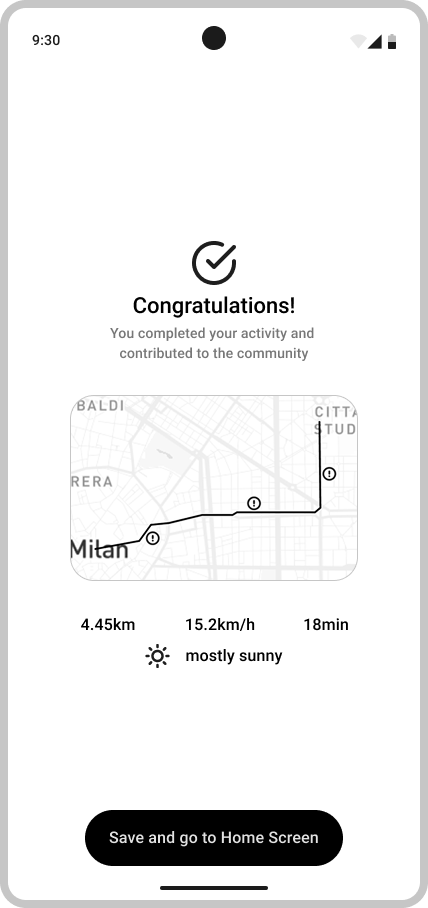
\includegraphics[width=0.75\textwidth]{RASD/source/images/UI/Congrats Screen.png}
        \caption{Congratulations Screen.}
        \label{fig:congratulation_screen}        
    \end{subfigure}
    \caption{Report and Congratulation Screens.}
    \label{fig:report_congrats_screen}
\end{figure}

\paragraph{Profile Screen}
In this screen the user can see his personal information and the number of activities and contributions he has made. Also, he can change his preferences via the toggle button or delete his account via the trash button. This screen is reserved to \underline{registered users only}.

\begin{figure}[H]
    \centering
    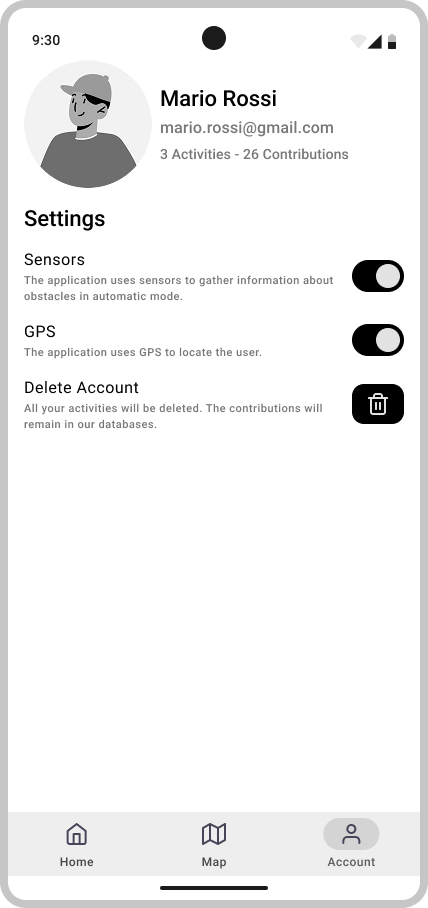
\includegraphics[width=0.25\linewidth]{RASD/source/images/UI/Profile Screen.png}
    \caption{Profile Screen.}
    \label{fig:profile_screen}
\end{figure}

\subsubsection{Hardware Interfaces}
The BBP system is a mobile application, requiring only a device with Android or iOS operating system installed. The device must have integrated sensors, GPS and internet access in order to allow the software to properly run.

\subsubsection{Software Interfaces}
The BBP system relies on the following software interfaces:
\begin{itemize}
    \item Weather API: the acquired data about the biking trip is enriched with weather information gathered from an external service.
    \item Map API: the BBP software must allow the user to visualize his current position in a virtual map, to show on the map different biking trips connecting the departure to the destination point, and allow the user to use the map to navigate through his journey. The application relies on an external map provider to gather this geographical information.  
\end{itemize}

\subsubsection{Communication Interfaces}
The BBP system as well as gathering external weather and map information, must also query all the needed data about roads, obstacles and registered users from the centralized database. The communication with the back-end must be secure and encrypted, especially for sensitive user data, such as name, surname email and password, so the HTTPS protocol is used. The data is then transferred using the JSON format.

\subsection{Functional Requirements}

\paragraph{Account and Access Management}
\begin{itemize}
    \item R1: The system shall allow biker to create an account.
    \item R2: The system shall allow registered users to log in.
    \item R3: The system shall allow registered users to update information in their profile.
    \item R4: The system shall allow registered users to delete their account.
\end{itemize}

\paragraph{Bike Path Discovery and Visualisation}
\begin{itemize}
    \item R5: The system shall allow users to browse the inventory of paths,
    \item R6: The system shall allow users to visualise available bike paths on a map provided by an external map service.
\end{itemize}

\paragraph{Trip Planning and Route Recommendation}
\begin{itemize}
    \item R7: The system shall allow registered users to plan a bike trip by storing it among planned trips,
    \item R8: The system shall allow the user to specify a starting and ending point in order to retrieve all the possible path between them.
    \item R9: In case a registered user has provided a departure and a destination point, the system shall return the possible paths ordered based on their scores.
\end{itemize}

\paragraph{Trip Tracking, History and Performance Analytics}
\begin{itemize}
    \item R10: The system shall allow registered users to record their trips.
    \item R11: The system shall provide registered users with statistics about their cycling performance.
    \item R12: The system shall allow registered users to view all the non deleted past trips.
    \item R13: The system shall allow registered users to delete trips from their trip history.
    \item R14: The system shall allow registered users to enable or disable automatic trip tracking. 
\end{itemize}

\paragraph{Reporting, Validation and Publication of Path Information}
\begin{itemize}
    \item R15: The system shall allow registered users to manually produce a report.
    \item R16: The system shall allow registered users to automatically produce a report.
    \item R17: The system shall allow registered users to review and validate reports produced automatically. 
    \item R18: The system shall allow registered users to publish manual reports.
    \item R19: The system shall allow registered users to publish validated reports produced automatically.
\end{itemize}

\paragraph{Context Enrichment and Notifications}
\begin{itemize}
    \item R20: The system shall notify registered users with planned trips when relevant weather conditions affecting the trip exceed a predefined severity threshold.
    \item R21: The system shall notify registered users with planned trips when obstacles along the associated path exceed a predefined severity threshold.
    \item R22: The system shall enrich trips in the inventory with meteorological information retrieved from an external weather service when available
\end{itemize}

\subsubsection{Use Case Diagram}
\begin{figure}[H]
    \centering
    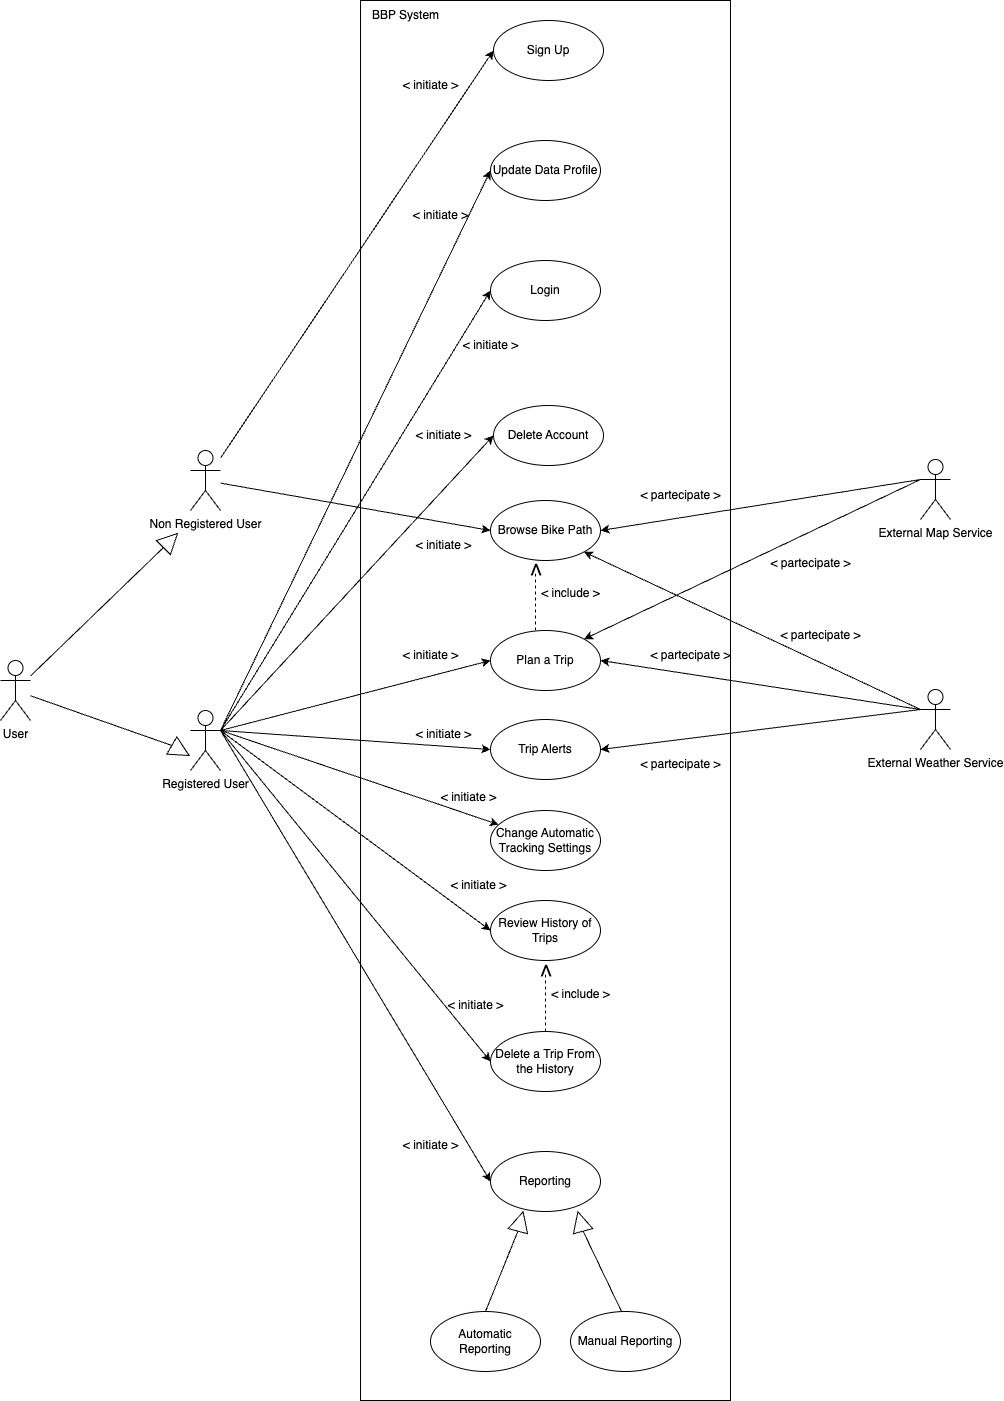
\includegraphics[width=0.65\linewidth]{RASD/source/images/diagrams/use_case_diagram.jpeg}
    \caption{Use Case Diagram.}
    \label{fig:use_case_diagram}
\end{figure}

\subsubsection{Use Cases}
% -----------------------------------------------------------------------------------------------------------------------
\noindent
\textbf{UC1: User Registration} 

\begin{table}[H]
    \centering
    \renewcommand{\arraystretch}{1.3}
    \begin{tabular}{|p{0.25\textwidth}|p{0.75\textwidth}|}
        \hline
        Name & \textbf{User Registration} \\
        \hline
        Actors & Non-Registered User. \\
        \hline
        Entry Condition & The user has access to the BBP system. \\
        \hline
        Event Flows & \begin{itemize}[topsep=0pt, partopsep=0pt, leftmargin=*]
            \item The user requests to create an account.
            \item The system requests registration data.
            \item The user provides registration data.
            \item The system validates the data and creates the account.
         \end{itemize} \\
        \hline
        Exit Condition & The user successfully registered to the platform. \\
        \hline
        Exception & \begin{itemize}[topsep=0pt, partopsep=0pt, leftmargin=*]
            \item Account already exists with associated email.
            \item Provided data is invalid.
        \end{itemize} \\
        \hline
        Special Requirements & Privacy: GDPR compliance for personal data handling, password storage \\
        \hline
    \end{tabular}
\end{table}

% -----------------------------------------------------------------------------------------------------------------------
\vspace{12pt}
\noindent
\textbf{UC2: User Login}

\begin{table}[H]
    \centering
    \renewcommand{\arraystretch}{1.3}
    \begin{tabular}{|p{0.25\textwidth}|p{0.75\textwidth}|}
        \hline
        Name & \textbf{User Login} \\
        \hline
        Actors & Registered User. \\
        \hline
        Entry Condition & A registered account exists. \\
        \hline
        Event Flows & \begin{itemize}[topsep=0pt, partopsep=0pt, leftmargin=*]
            \item The user requests to log in.
            \item The system requests credentials.
            \item The user provides credentials.
            \item The system authenticates the user and grants access.
        \end{itemize} \\
        \hline
        Exit Condition & The user is authenticated and has access to registered features. \\
        \hline
        Exception & \begin{itemize}[topsep=0pt, partopsep=0pt, leftmargin=*]
            \item Account not available (deleted/blocked).
            \item Invalid credentials.
        \end{itemize} \\
        \hline
        Special Requirements & Security: Authentication and session handling \\
        \hline
    \end{tabular}
\end{table}

% -----------------------------------------------------------------------------------------------------------------------
\newpage
\noindent
\textbf{UC3: Update Profile Data}

\begin{table}[H]
    \centering
    \renewcommand{\arraystretch}{1.3}
    \begin{tabular}{|p{0.25\textwidth}|p{0.75\textwidth}|}
        \hline
        Name & \textbf{Update Profile Data} \\
        \hline
        Actors & Registered User. \\
        \hline
        Entry Condition & The user is authenticated. \\
        \hline
        Event Flows & \begin{itemize}[topsep=0pt, partopsep=0pt, leftmargin=*]
            \item The user requests to update profile information.
            \item The system displays current profile data (conceptually: makes them available for editing).
            \item The user submits updated data.
            \item The system validates and stores the updates.
        \end{itemize} \\
        \hline
        Exit Condition & User's profile data is updated. \\
        \hline
        Exception & \begin{itemize}[topsep=0pt, partopsep=0pt, leftmargin=*]
            \item Invalid new profile information.
        \end{itemize} \\
        \hline
        Special Requirements & Privacy: GDPR compliance for personal data handling, password storage \\
        \hline
    \end{tabular}
\end{table}

% -----------------------------------------------------------------------------------------------------------------------
\vspace{12pt}
\noindent
\textbf{UC4: Delete Account}

\begin{table}[H]
    \centering
    \renewcommand{\arraystretch}{1.3}
    \begin{tabular}{|p{0.25\textwidth}|p{0.75\textwidth}|}
        \hline
        Name & \textbf{Delete Account} \\
        \hline
        Actors & Registered User. \\
        \hline
        Entry Condition & The user is authenticated. \\
        \hline
        Event Flows & \begin{itemize}[topsep=0pt, partopsep=0pt, leftmargin=*]
            \item The user requests account deletion.
            \item The system performs the deletion according to retention rules.
            \item The system revokes access.
        \end{itemize} \\
        \hline
        Exit Condition & The account is deleted and the user becomes non-registered. \\
        \hline
        Exception & \\
        \hline
        Special Requirements & Privacy: GDPR compliance for personal data handling, password storage \\
        \hline
    \end{tabular}
\end{table}

% -----------------------------------------------------------------------------------------------------------------------
\newpage
\noindent
\textbf{UC5: Browse Bike Paths}

\begin{table}[H]
    \centering
    \renewcommand{\arraystretch}{1.3}
    \begin{tabular}{|p{0.25\textwidth}|p{0.75\textwidth}|}
        \hline
        Name & \textbf{Delete Account} \\
        \hline
        Actors & \begin{enumerate}[topsep=0pt, partopsep=0pt, leftmargin=*]
            \item User (Registered or not).
            \item External Map Service, External Weather Service.
        \end{enumerate} \\
        \hline
        Entry Condition & The user has access to the BBP system \\
        \hline
        Event Flows & \begin{itemize}[topsep=0pt, partopsep=0pt, leftmargin=*]
            \item The user requests to explore available bike paths.
            \item (Optional) The user provides departure–destination points.
            \item The system retrieves the matching paths.
            \item The system provides path information (status, score, obstacles/reports summary).
            \item (Optional) The system retrieves and shows map representation via the external map service.
            \item (Optional) The system retrieves and shows weather information for the relevant area/time.
        \end{itemize} \\
        \hline
        Exit Condition & The user explores available paths and their information. \\
        \hline
        Exception & No paths match the request. \\
        \hline
        Special Requirements & Compatibility: interoperability with external services (map/weather systems). \\
        \hline
    \end{tabular}
\end{table}

% -----------------------------------------------------------------------------------------------------------------------
\newpage
\noindent
\textbf{UC6: Plan Trips}

\begin{table}[H]
    \centering
    \renewcommand{\arraystretch}{1.3}
    \begin{tabular}{|p{0.25\textwidth}|p{0.75\textwidth}|}
        \hline
        Name & \textbf{Plan Trips} \\
        \hline
        Actors & \begin{enumerate}[topsep=0pt, partopsep=0pt, leftmargin=*]
            \item Registered User.
            \item External Map Service, External Weather Service.
        \end{enumerate} \\
        \hline
        Entry Condition & The user is authenticated. \\
        \hline
        Event Flows & \begin{itemize}[topsep=0pt, partopsep=0pt, leftmargin=*]
            \item The user requests to plan a new trip.
            \item The user selects a bike path
            \item The system stores the trip in the planned trips list.
            \item (Optional) The system enriches the planned trip with available weather information.
        \end{itemize} \\
        \hline
        Exit Condition & A planned trip is stored and managed by the system. \\
        \hline
        Exception & \begin{itemize}[topsep=0pt, partopsep=0pt, leftmargin=*]
            \item Selected path becomes unavailable during planning.
            \item System error preventing trip storage.
        \end{itemize} \\
        \hline
        Special Requirements & Performance: time behaviour.\\
        \hline
    \end{tabular}
\end{table}

% -----------------------------------------------------------------------------------------------------------------------
\vspace{12pt}
\noindent
\textbf{UC7: Change Automatic Tracking Settings}

\begin{table}[H]
    \centering
    \renewcommand{\arraystretch}{1.3}
    \begin{tabular}{|p{0.25\textwidth}|p{0.75\textwidth}|}
        \hline
        Name & \textbf{Change Automatic Tracking Settings} \\
        \hline
        Actors & \begin{enumerate}[topsep=0pt, partopsep=0pt, leftmargin=*]
            \item Registered User.
            \item User Device (sensors and GPS).
        \end{enumerate} \\
        \hline
        Entry Condition & he user is authenticated. \\
        \hline
        Event Flows & \begin{itemize}[topsep=0pt, partopsep=0pt, leftmargin=*]
            \item The user requests to enable or disable automatic trip tracking.
            \item The system stores the user’s tracking preference.
            \item (If enabling) the system requests to collect sensor/GPS data.
        \end{itemize} \\
        \hline
        Exit Condition & Tracking preference is updated. \\
        \hline
        Exception & \begin{itemize}[topsep=0pt, partopsep=0pt, leftmargin=*]
            \item User device does not support required sensors.
            \item User denies required permissions/consent.
        \end{itemize} \\
        \hline
        Special Requirements & Privacy: explicit consent for location/sensor tracking. \\
        \hline
    \end{tabular}
\end{table}

% -----------------------------------------------------------------------------------------------------------------------
\newpage
\noindent
\textbf{UC8: View History and Statistics of Completed Trips}

\begin{table}[H]
    \centering
    \renewcommand{\arraystretch}{1.3}
    \begin{tabular}{|p{0.25\textwidth}|p{0.75\textwidth}|}
        \hline
        Name & \textbf{View History and Statistics of Completed Trips} \\
        \hline
        Actors & Registered User \\
        \hline
        Entry Condition & he user is authenticated.\\
        \hline
        Event Flows & \begin{itemize}[topsep=0pt, partopsep=0pt, leftmargin=*]
            \item The user requests access to trip history.
            \item The system retrieves all non-deleted completed trips.
            \item The user selects a trip.
            \item The system provides the trip details and related statistics.
        \end{itemize} \\
        \hline
        Exit Condition & The user has reviewed past trips and their statistics\\
        \hline
        Exception & No trips exist in the history\\
        \hline
    \end{tabular}
\end{table}

% -----------------------------------------------------------------------------------------------------------------------
\vspace{12pt}
\noindent
\textbf{UC9: Delete Trips from History}

\begin{table}[H]
    \centering
    \renewcommand{\arraystretch}{1.3}
    \begin{tabular}{|p{0.25\textwidth}|p{0.75\textwidth}|}
        \hline
        Name & \textbf{Delete Trips from History} \\
        \hline
        Actors & Registered User. \\
        \hline
        Entry Condition & The user is authenticated and at least one trip exists in history. \\
        \hline
        Event Flows & \begin{itemize}[topsep=0pt, partopsep=0pt, leftmargin=*]
            \item The user requests deletion of a specific past trip.
            \item The system removes the trip from the user’s history (marks as deleted).
            \item The system updates any aggregated views/metrics to exclude deleted trips.
        \end{itemize} \\
        \hline
        Exit Condition & The selected trip is deleted from history. \\
        \hline
        Special Requirements & Data Consistency: deleted trips must not appear in global statistics and history views. \\
        \hline
    \end{tabular}
\end{table}

% -----------------------------------------------------------------------------------------------------------------------
\newpage
\noindent
\textbf{UC10: Manual Report}

\begin{table}[H]
    \centering
    \renewcommand{\arraystretch}{1.3}
    \begin{tabular}{|p{0.25\textwidth}|p{0.75\textwidth}|}
        \hline
        Name & \textbf{Manual Report} \\
        \hline
        Actors & Registered User. \\
        \hline
        Entry Condition & A trip has been completed. \\
        \hline
        Event Flows & \begin{itemize}[topsep=0pt, partopsep=0pt, leftmargin=*]
            \item The user requests to create a manual report about a planned bike path.
            \item The user provides report data (conditions, obstacles, notes) and request the publication
            \item The system stores the report and publishes it as public path information.
        \end{itemize} \\
        \hline
        Exit Condition & A manual report is published and contributes to path enrichment. \\
        \hline
        Exceptions & Report data is invalid or incomplete. \\
        \hline
    \end{tabular}
\end{table}

% -----------------------------------------------------------------------------------------------------------------------
\vspace{12pt}
\noindent
\textbf{UC11: Automatic Report}

\begin{table}[H]
    \centering
    \renewcommand{\arraystretch}{1.3}
    \begin{tabular}{|p{0.25\textwidth}|p{0.75\textwidth}|}
        \hline
        Name & \textbf{Automatic Report} \\
        \hline
        Actors & \begin{enumerate}[topsep=0pt, partopsep=0pt, leftmargin=*]
            \item Registered User. 
            \item User's Device (data source).
        \end{enumerate} \\
        \hline
        Entry Condition & A trip has been recorded with automatic tracking enabled. \\
        \hline
        Event Flows & \begin{itemize}[topsep=0pt, partopsep=0pt, leftmargin=*]
            \item The system generates an automatic report from collected trip data.
            \item The user requests to review the generated report.
            \item The user possibly corrects the report and confirm it
            \item The system marks the report as validated
            \item The user confirms the report and requests the publication
            \item The system publishes the report.
        \end{itemize} \\
        \hline
        Exit Condition & A validated automatic report is published. \\
        \hline
        Exceptions & \begin{itemize}[topsep=0pt, partopsep=0pt, leftmargin=*]
            \item Automatic tracking was not enabled: no automatic report exists.
            \item User discards the report: the report is not published.
        \end{itemize} \\
        \hline
        Special requirements & Reliability: fault tolerance (incomplete data coming from device sensors).\\
        \hline
    \end{tabular}
\end{table}

% -----------------------------------------------------------------------------------------------------------------------
\newpage
\noindent
\textbf{UC12: Receive Trip Alerts}

\begin{table}[H]
    \centering
    \renewcommand{\arraystretch}{1.3}
    \begin{tabular}{|p{0.25\textwidth}|p{0.75\textwidth}|}
        \hline
        Name & \textbf{Receive Trip Alerts} \\
        \hline
        Actors & \begin{enumerate}[topsep=0pt, partopsep=0pt, leftmargin=*]
            \item Registered User. 
            \item External Weather Service, Other (reporting) Users.
        \end{enumerate} \\
        \hline
        Entry Condition & At least one planned trip exists. \\
        \hline
        Event Flows & \begin{itemize}[topsep=0pt, partopsep=0pt, leftmargin=*]
            \item The system detects relevant changes affecting a planned trip (e.g., adverse weather severity threshold exceeded; obstacle severity threshold exceeded).
            \item The system notifies the user.
        \end{itemize} \\
        \hline
        Exit Condition & The user receives the alert information \\
        \hline
        Exceptions & External weather service unavailable (weather alerts may be delayed/unavailable). \\
        \hline
    \end{tabular}
\end{table}



\subsubsection{Sequence Diagrams}

\noindent
\textbf{User Registration}
\begin{figure}[H]
    \centering
    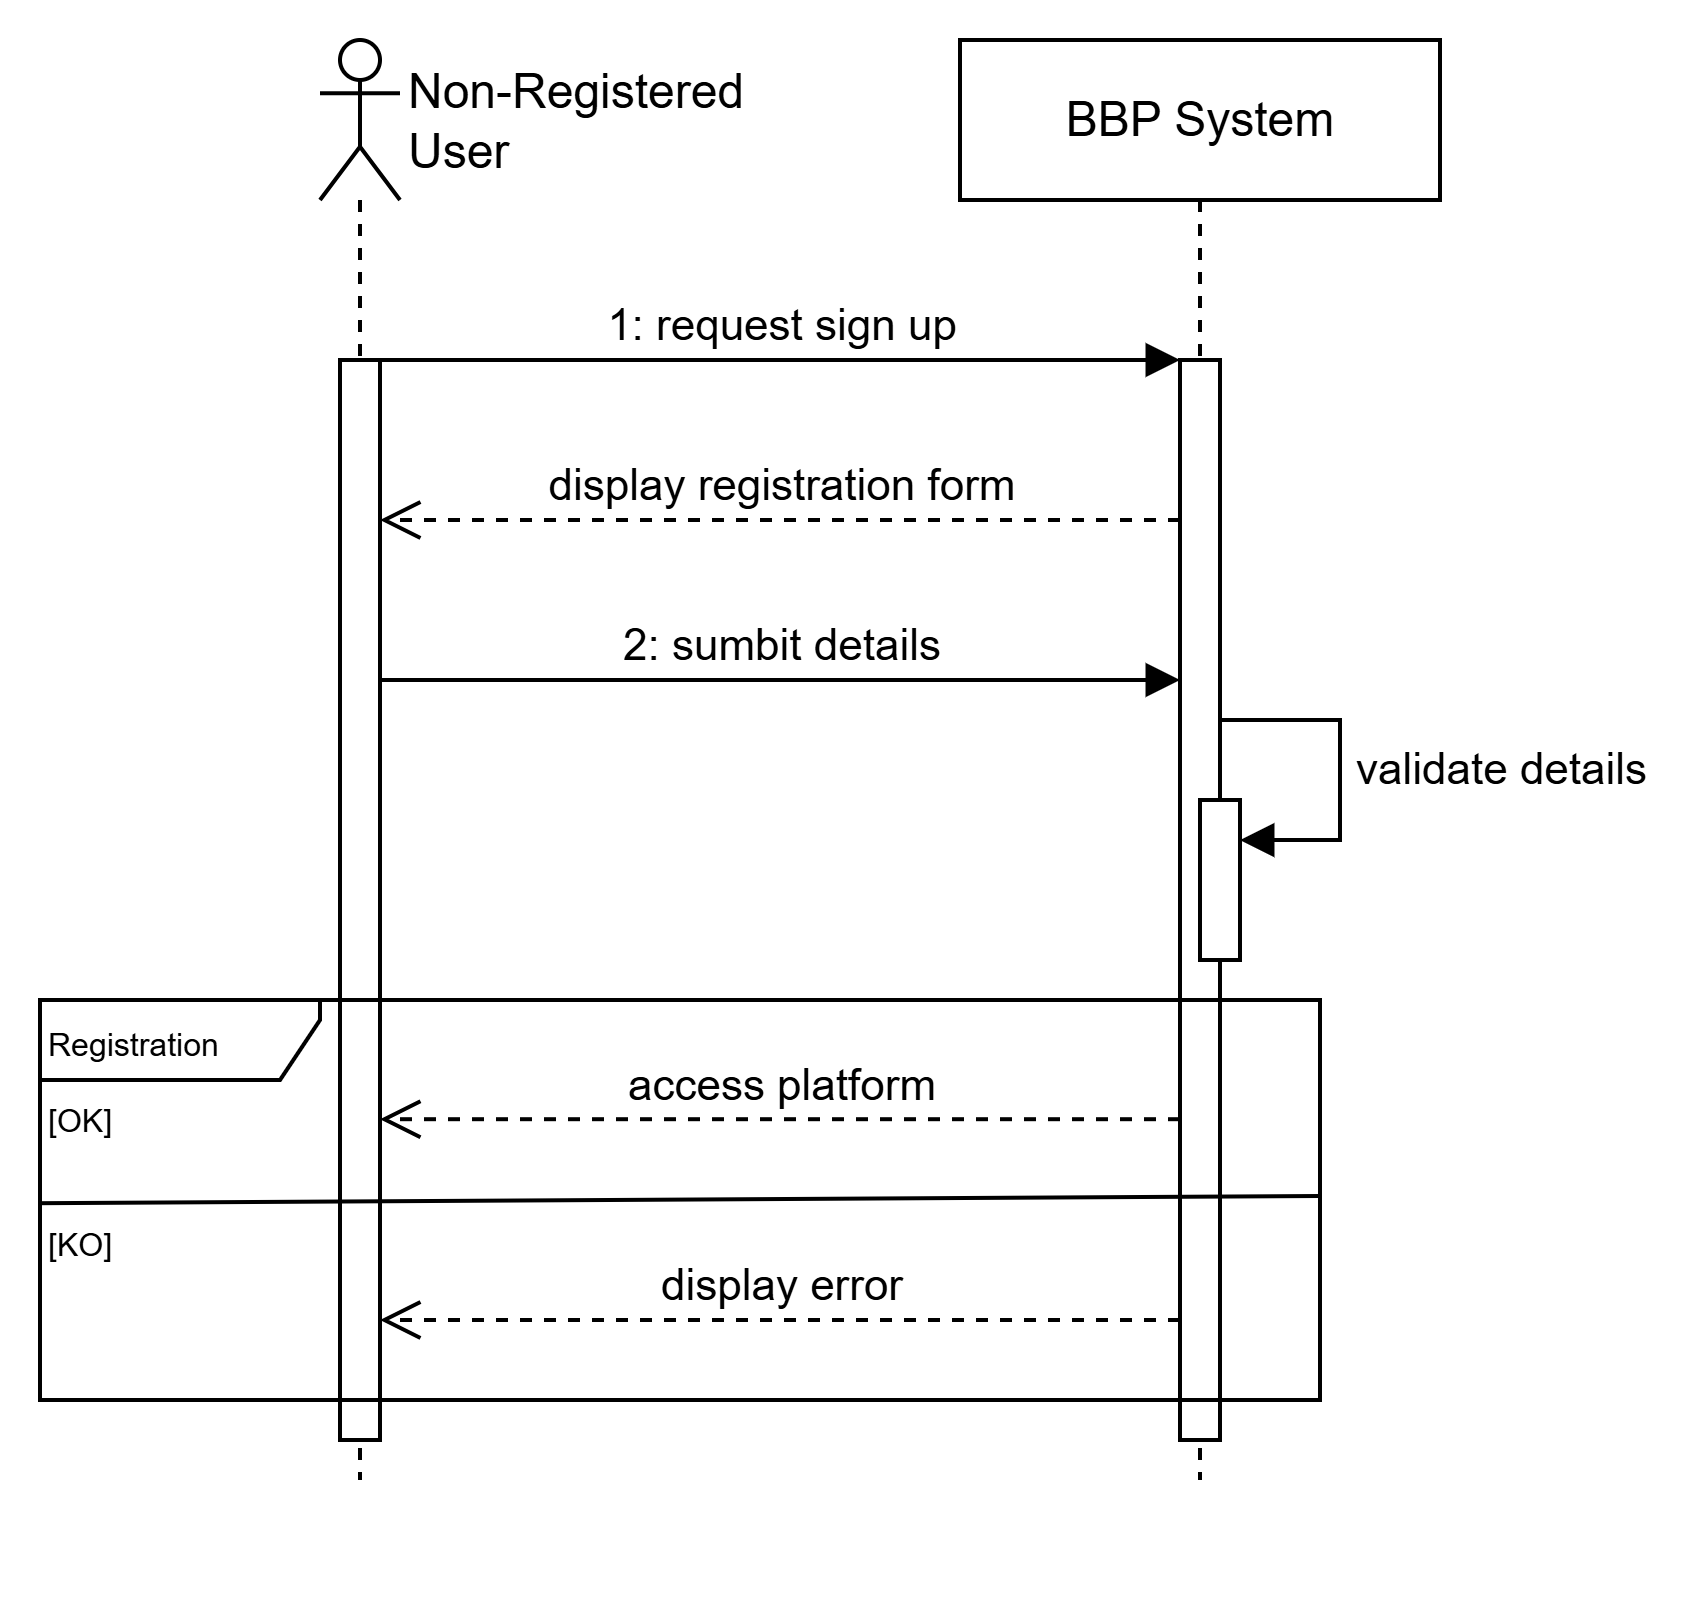
\includegraphics[width=0.5\linewidth]{RASD/source/images/diagrams/sd_registration.png}
    \caption{User Registration Sequence Diagram.}
    \label{fig:sd_registration}
\end{figure}

\newpage
\noindent
\textbf{User Log In}
\begin{figure}[H]
    \centering
    
\includegraphics[width=0.5\linewidth]{RASD//source//images//diagrams/sd_login.png}
    \caption{User Log In Sequence Diagram.}
    \label{fig:sd_login}
\end{figure}

\noindent
\textbf{Update Profile Data}
\begin{figure}[H]
    \centering
    
\includegraphics[width=0.5\linewidth]{RASD//source//images//diagrams/sd_update_profile.png}
    \caption{Update Profile Data Sequence Diagram.}
    \label{fig:sd_profile_update}
\end{figure}

\newpage
\noindent
\textbf{Delete Account}
\begin{figure}[H]
    \centering
    
\includegraphics[width=0.5\linewidth]{RASD//source//images//diagrams/sd_delete_account.png}
    \caption{Delete Account Sequence Diagram.}
    \label{fig:sd_delete_account}
\end{figure}

\noindent
\textbf{Browse Bike Paths}
\begin{figure}[H]
    \centering
    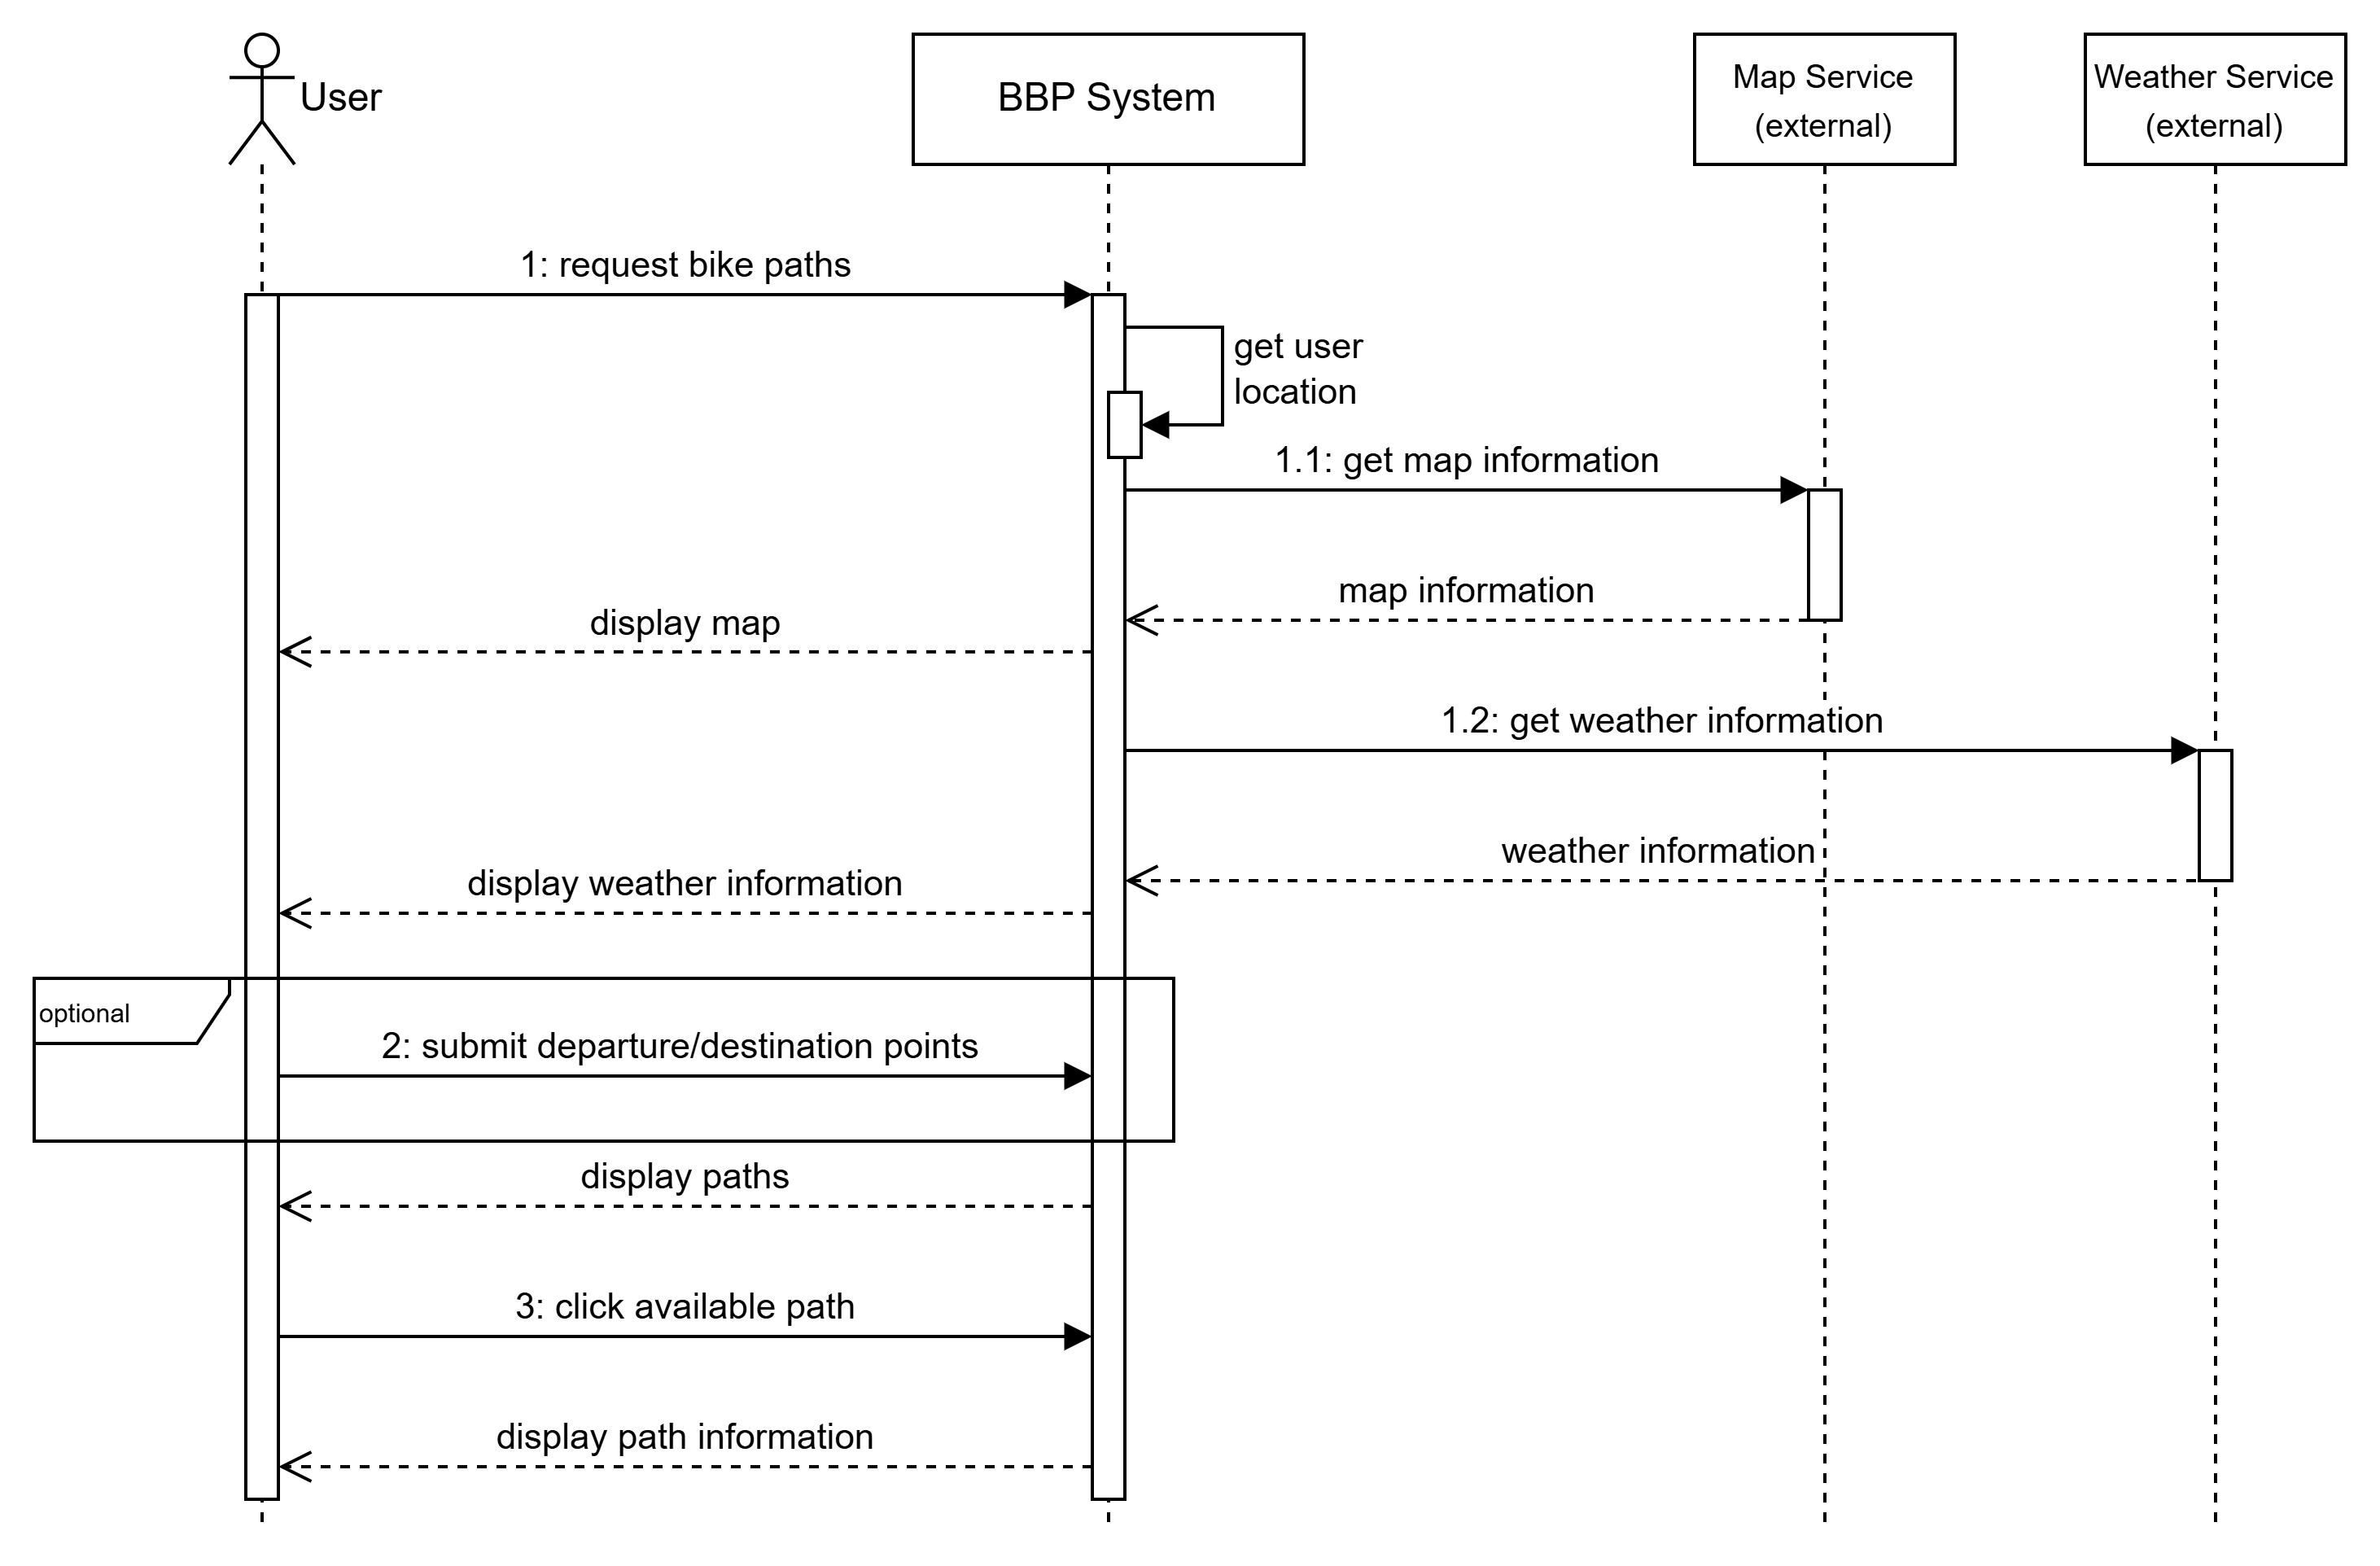
\includegraphics[width=0.75\linewidth]{RASD//source//images//diagrams/sd_browse_bike_paths.png}
    \caption{Browse Bike Paths Sequence Diagram.}
    \label{fig:sd_browse_bike_paths}
\end{figure}

\newpage
\noindent
\textbf{Plan Trip}
\begin{figure}[H]
    \centering
    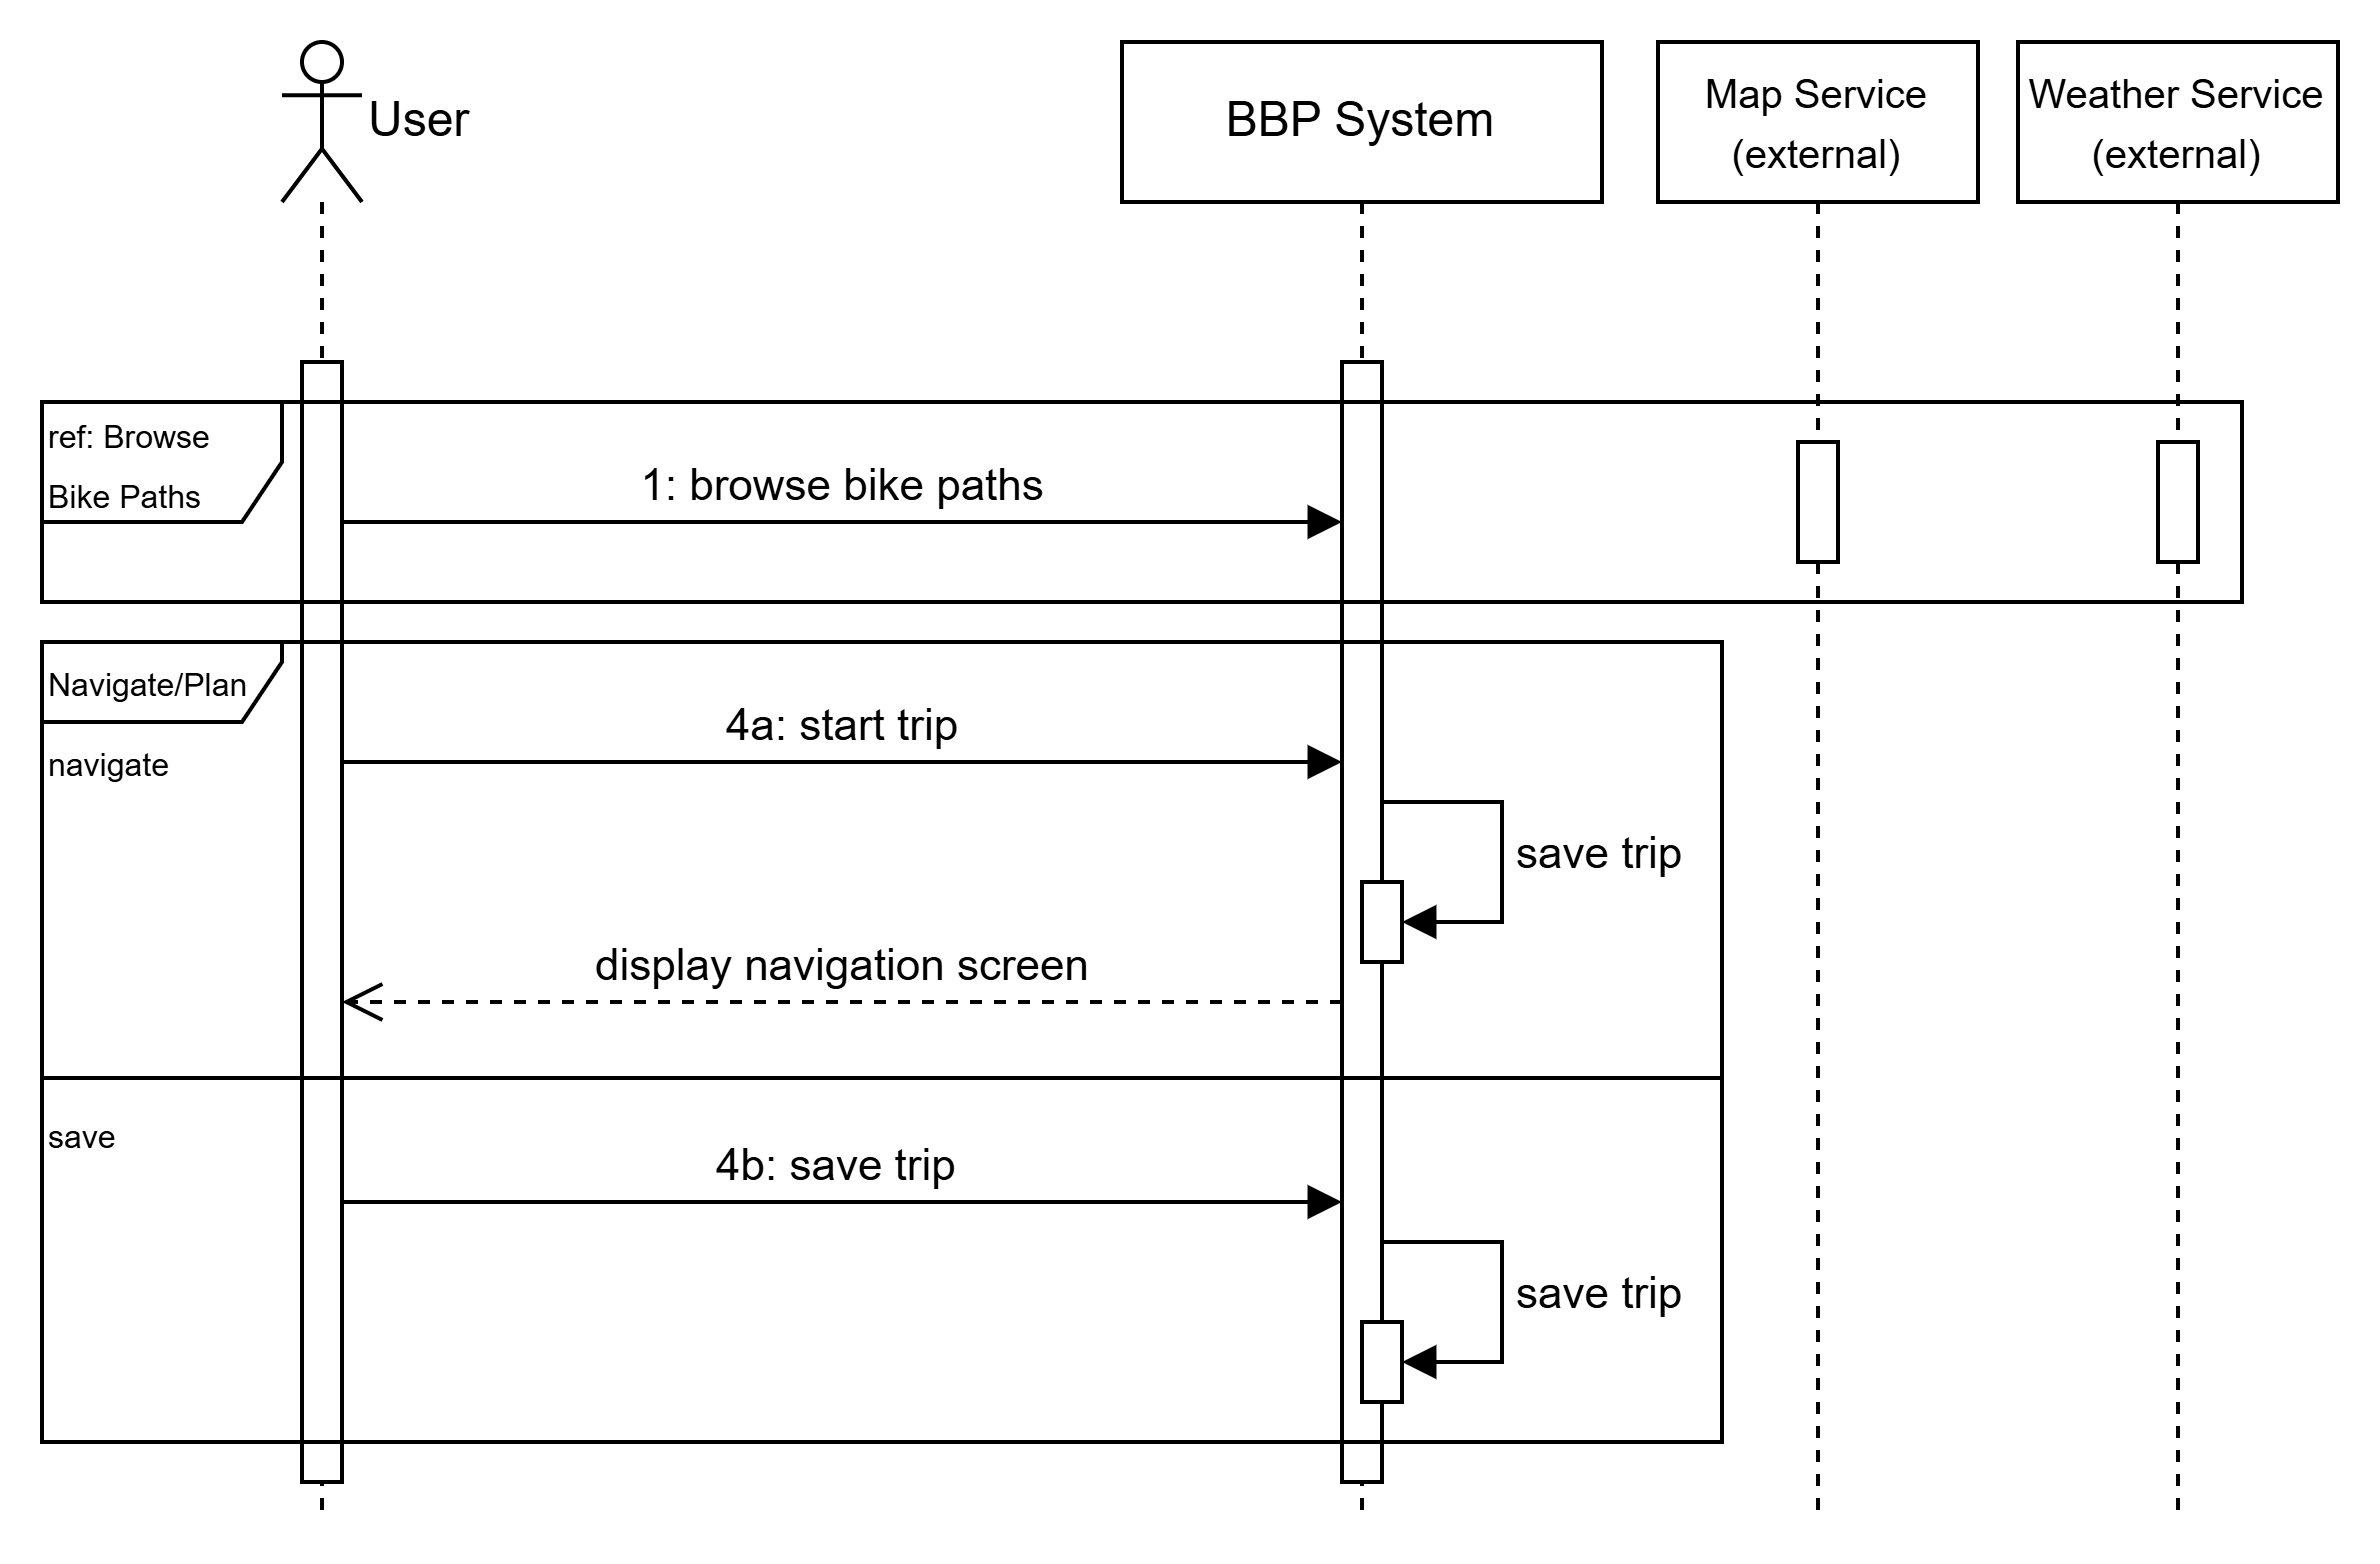
\includegraphics[width=0.75\linewidth]{RASD//source//images//diagrams/sd_plan_trip.png}
    \caption{Plan Trip Sequence Diagram.}
    \label{fig:sd_plan_trip}
\end{figure}

\noindent
\textbf{Change Sensor Preferences}
\begin{figure}[H]
    \centering
    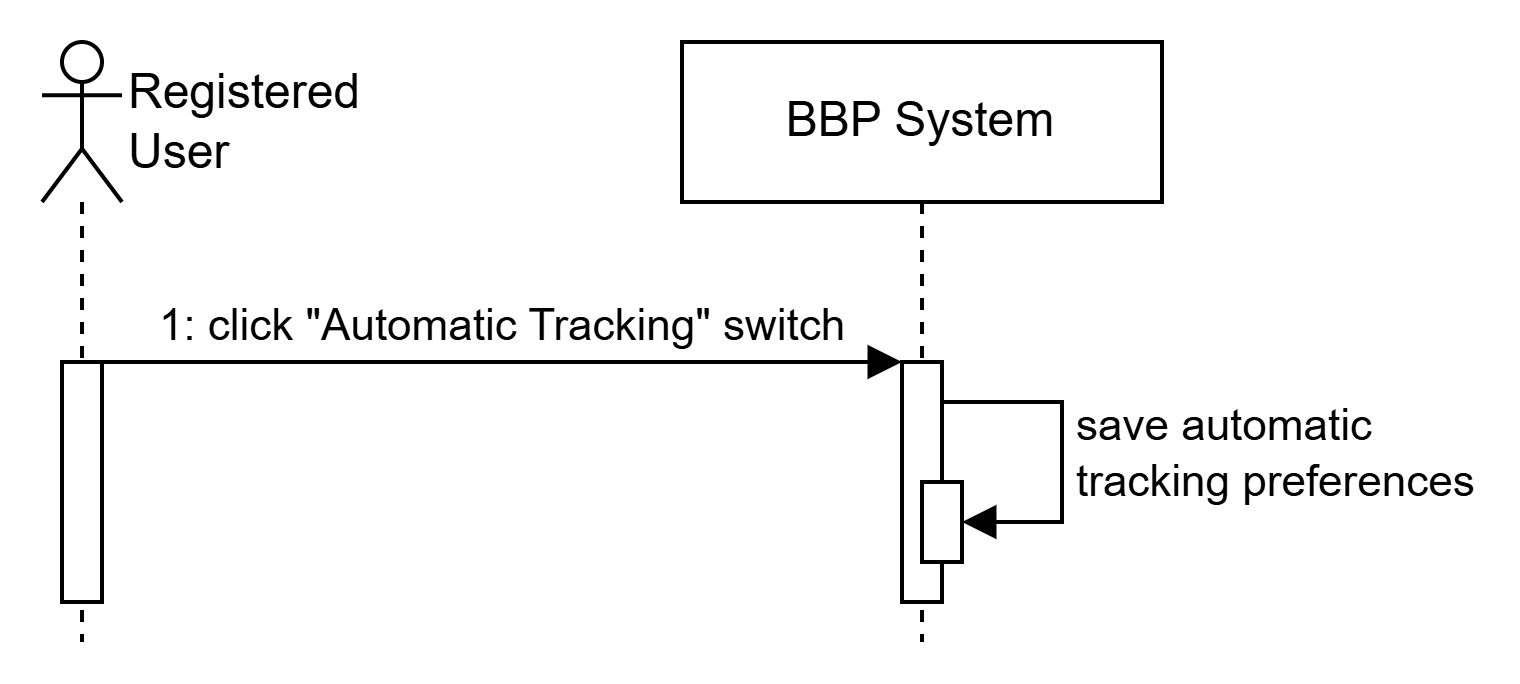
\includegraphics[width=0.5\linewidth]{RASD//source//images//diagrams/sd_change_sensor_preferences.png}
    \caption{Change Sensor Preferences Sequence Diagram.}
    \label{fig:sd_change_sensor_preferences}
\end{figure}

\newpage
\noindent
\textbf{View Trip Details and Statistics}
\begin{figure}[H]
    \centering
    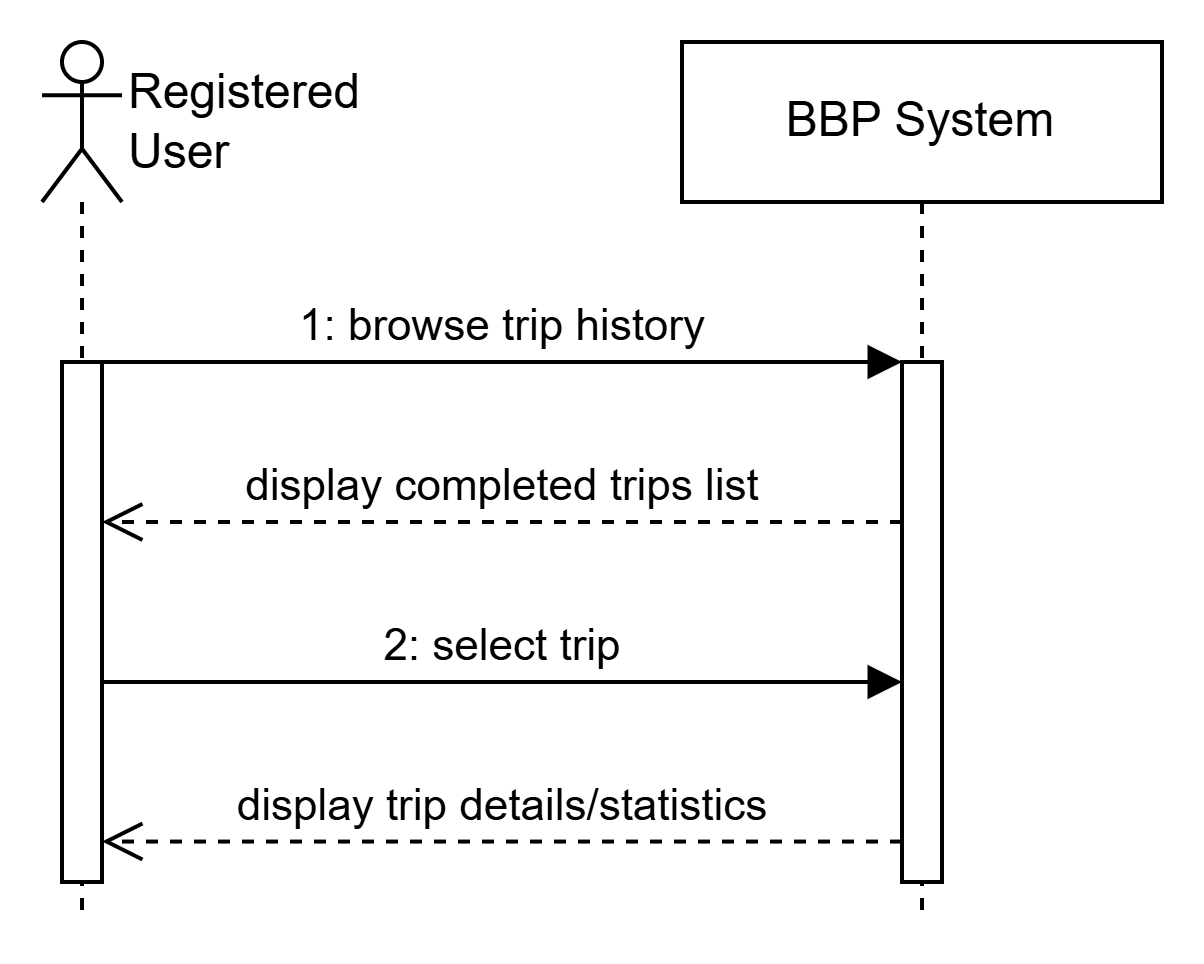
\includegraphics[width=0.4\linewidth]{RASD//source//images//diagrams/sd_trip_details.png}
    \caption{View Trip Details Sequence Diagram.}
    \label{fig:sd_trip_details}
\end{figure}

\noindent
\textbf{Delete Trip}
\begin{figure}[H]
    \centering
    
\includegraphics[width=0.5\linewidth]{RASD//source//images//diagrams/sd_delete_trip.png}
    \caption{Delete Trip Sequence Diagram.}
    \label{fig:sd_delete_trip}
\end{figure}

\newpage
\noindent
\textbf{Manual Report}
\begin{figure}[H]
    \centering
    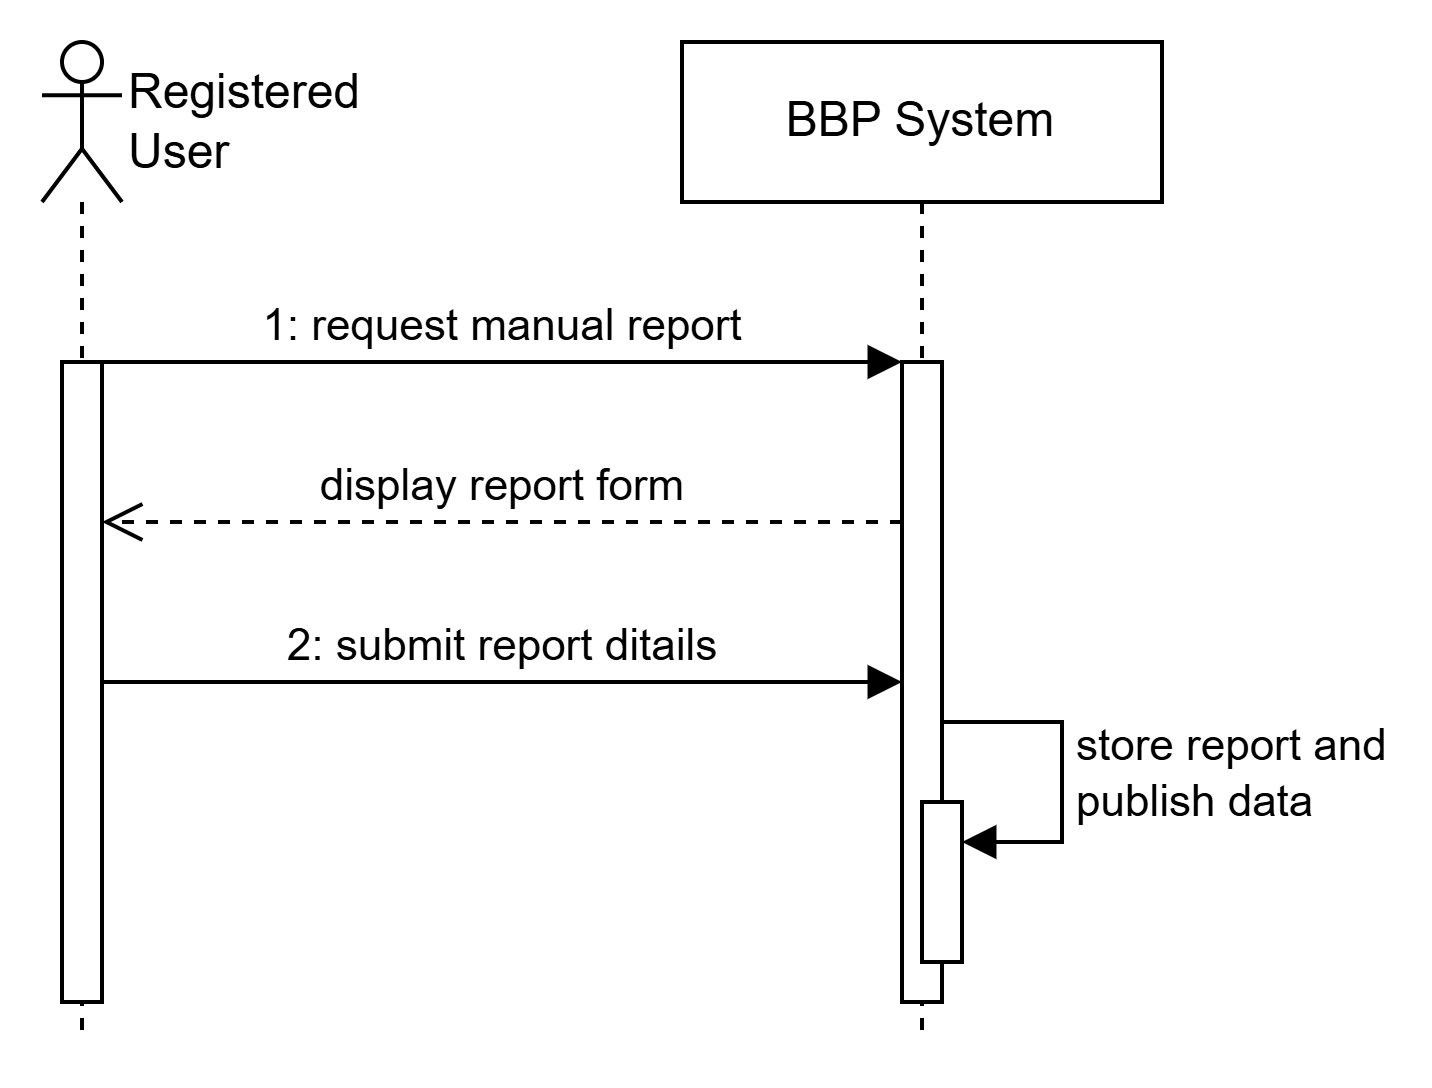
\includegraphics[width=0.5\linewidth]{RASD//source//images//diagrams/sd_manual_report.png}
    \caption{Manual Report Sequence Diagram.}
    \label{fig:sd_manual_report}
\end{figure}

\noindent
\textbf{Automatic Report}
\begin{figure}[H]
    \centering
    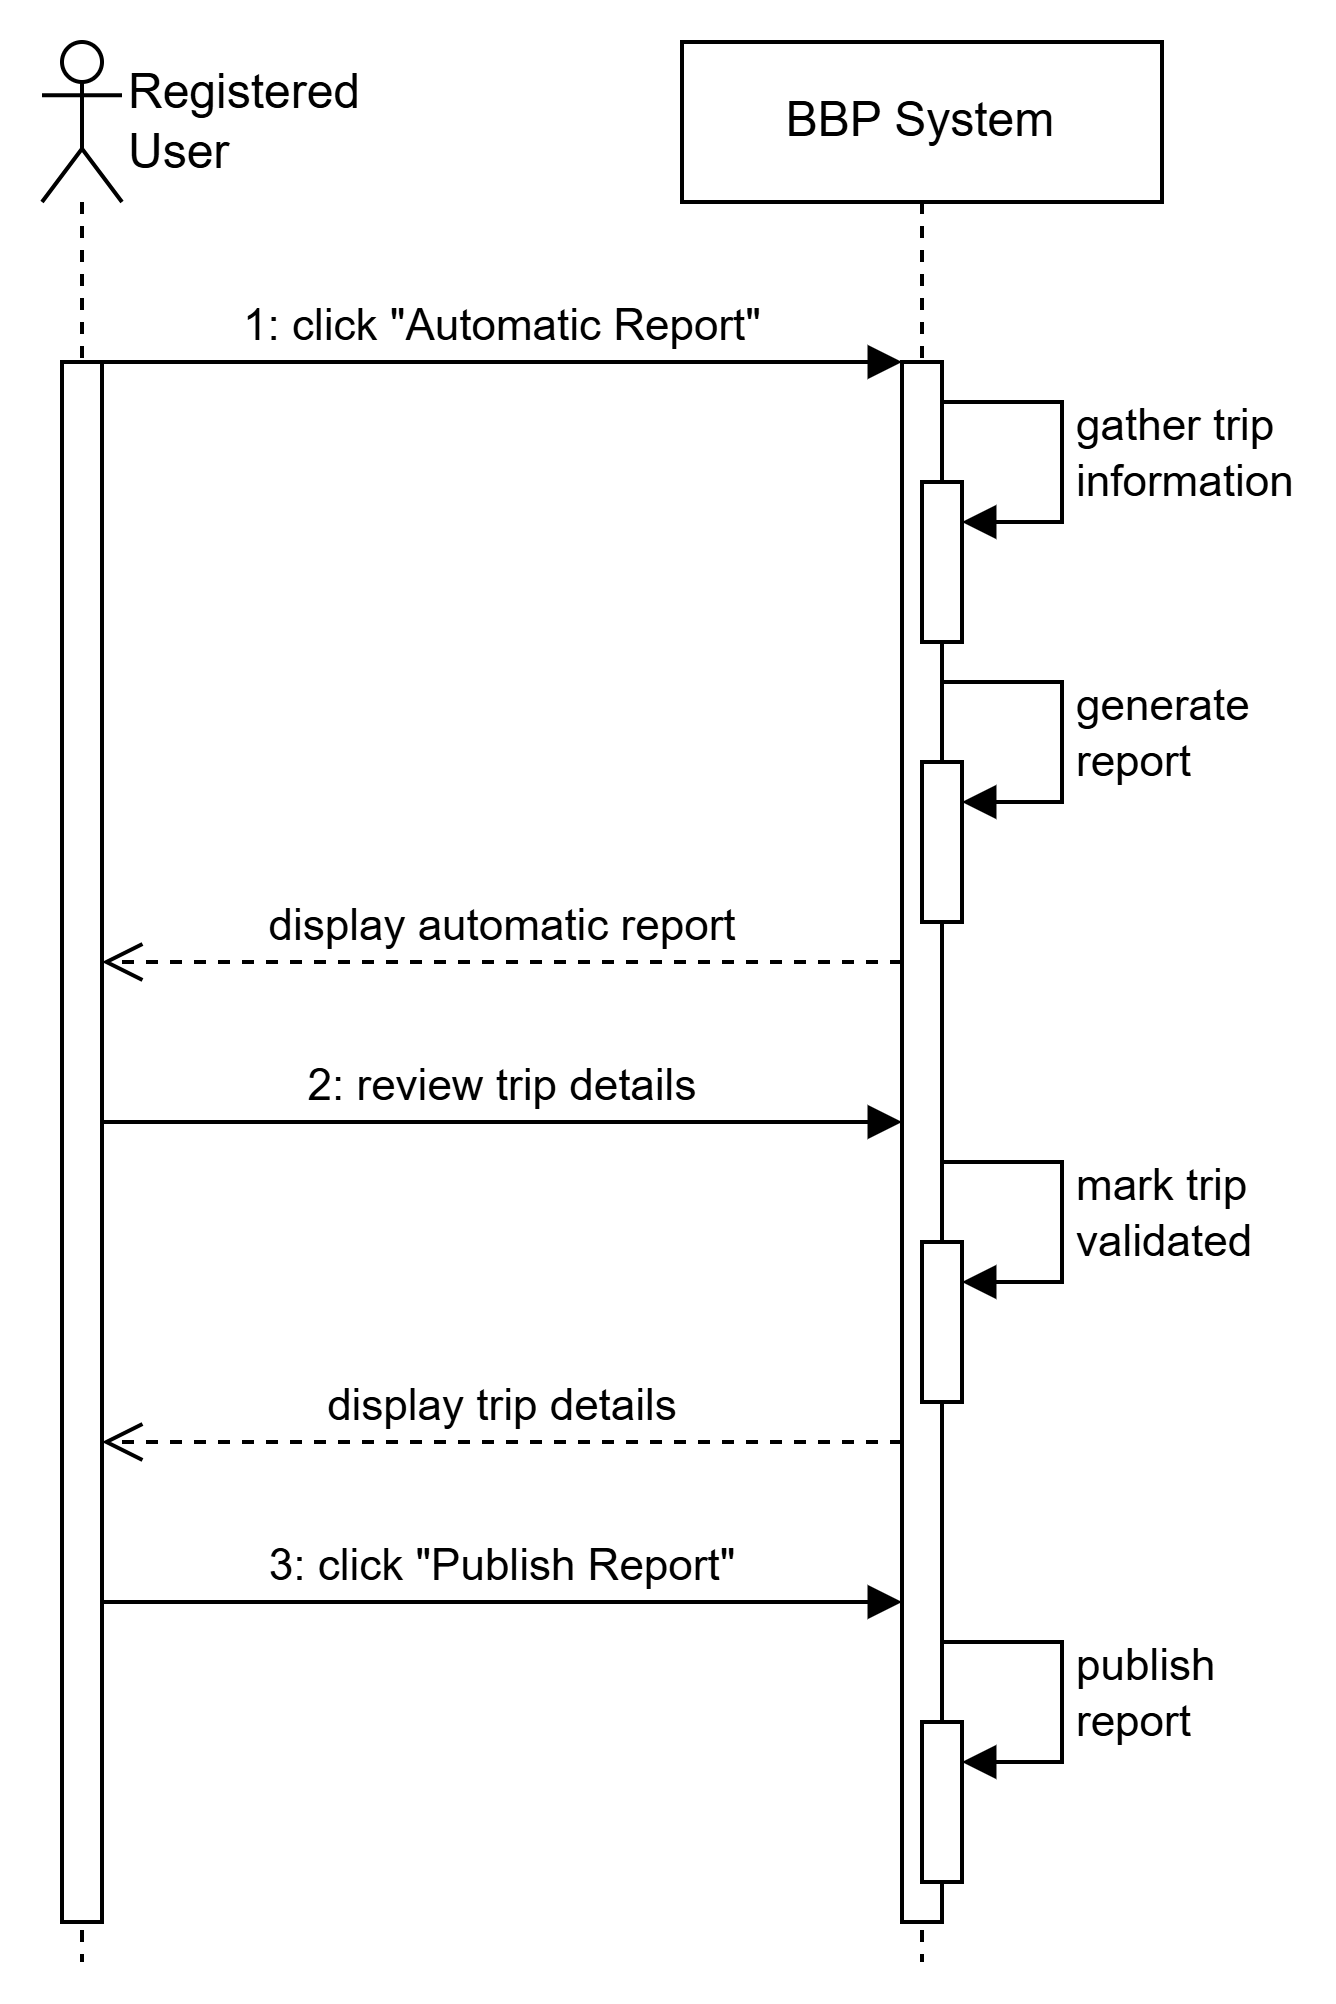
\includegraphics[width=0.4\linewidth]{RASD//source//images//diagrams/sd_automatic_report.png}
    \caption{Manual Report Sequence Diagram.}
    \label{fig:sd_automatic_report}
\end{figure}

\newpage
\noindent
\textbf{Receive Trip Alerts}
\begin{figure}[H]
    \centering
    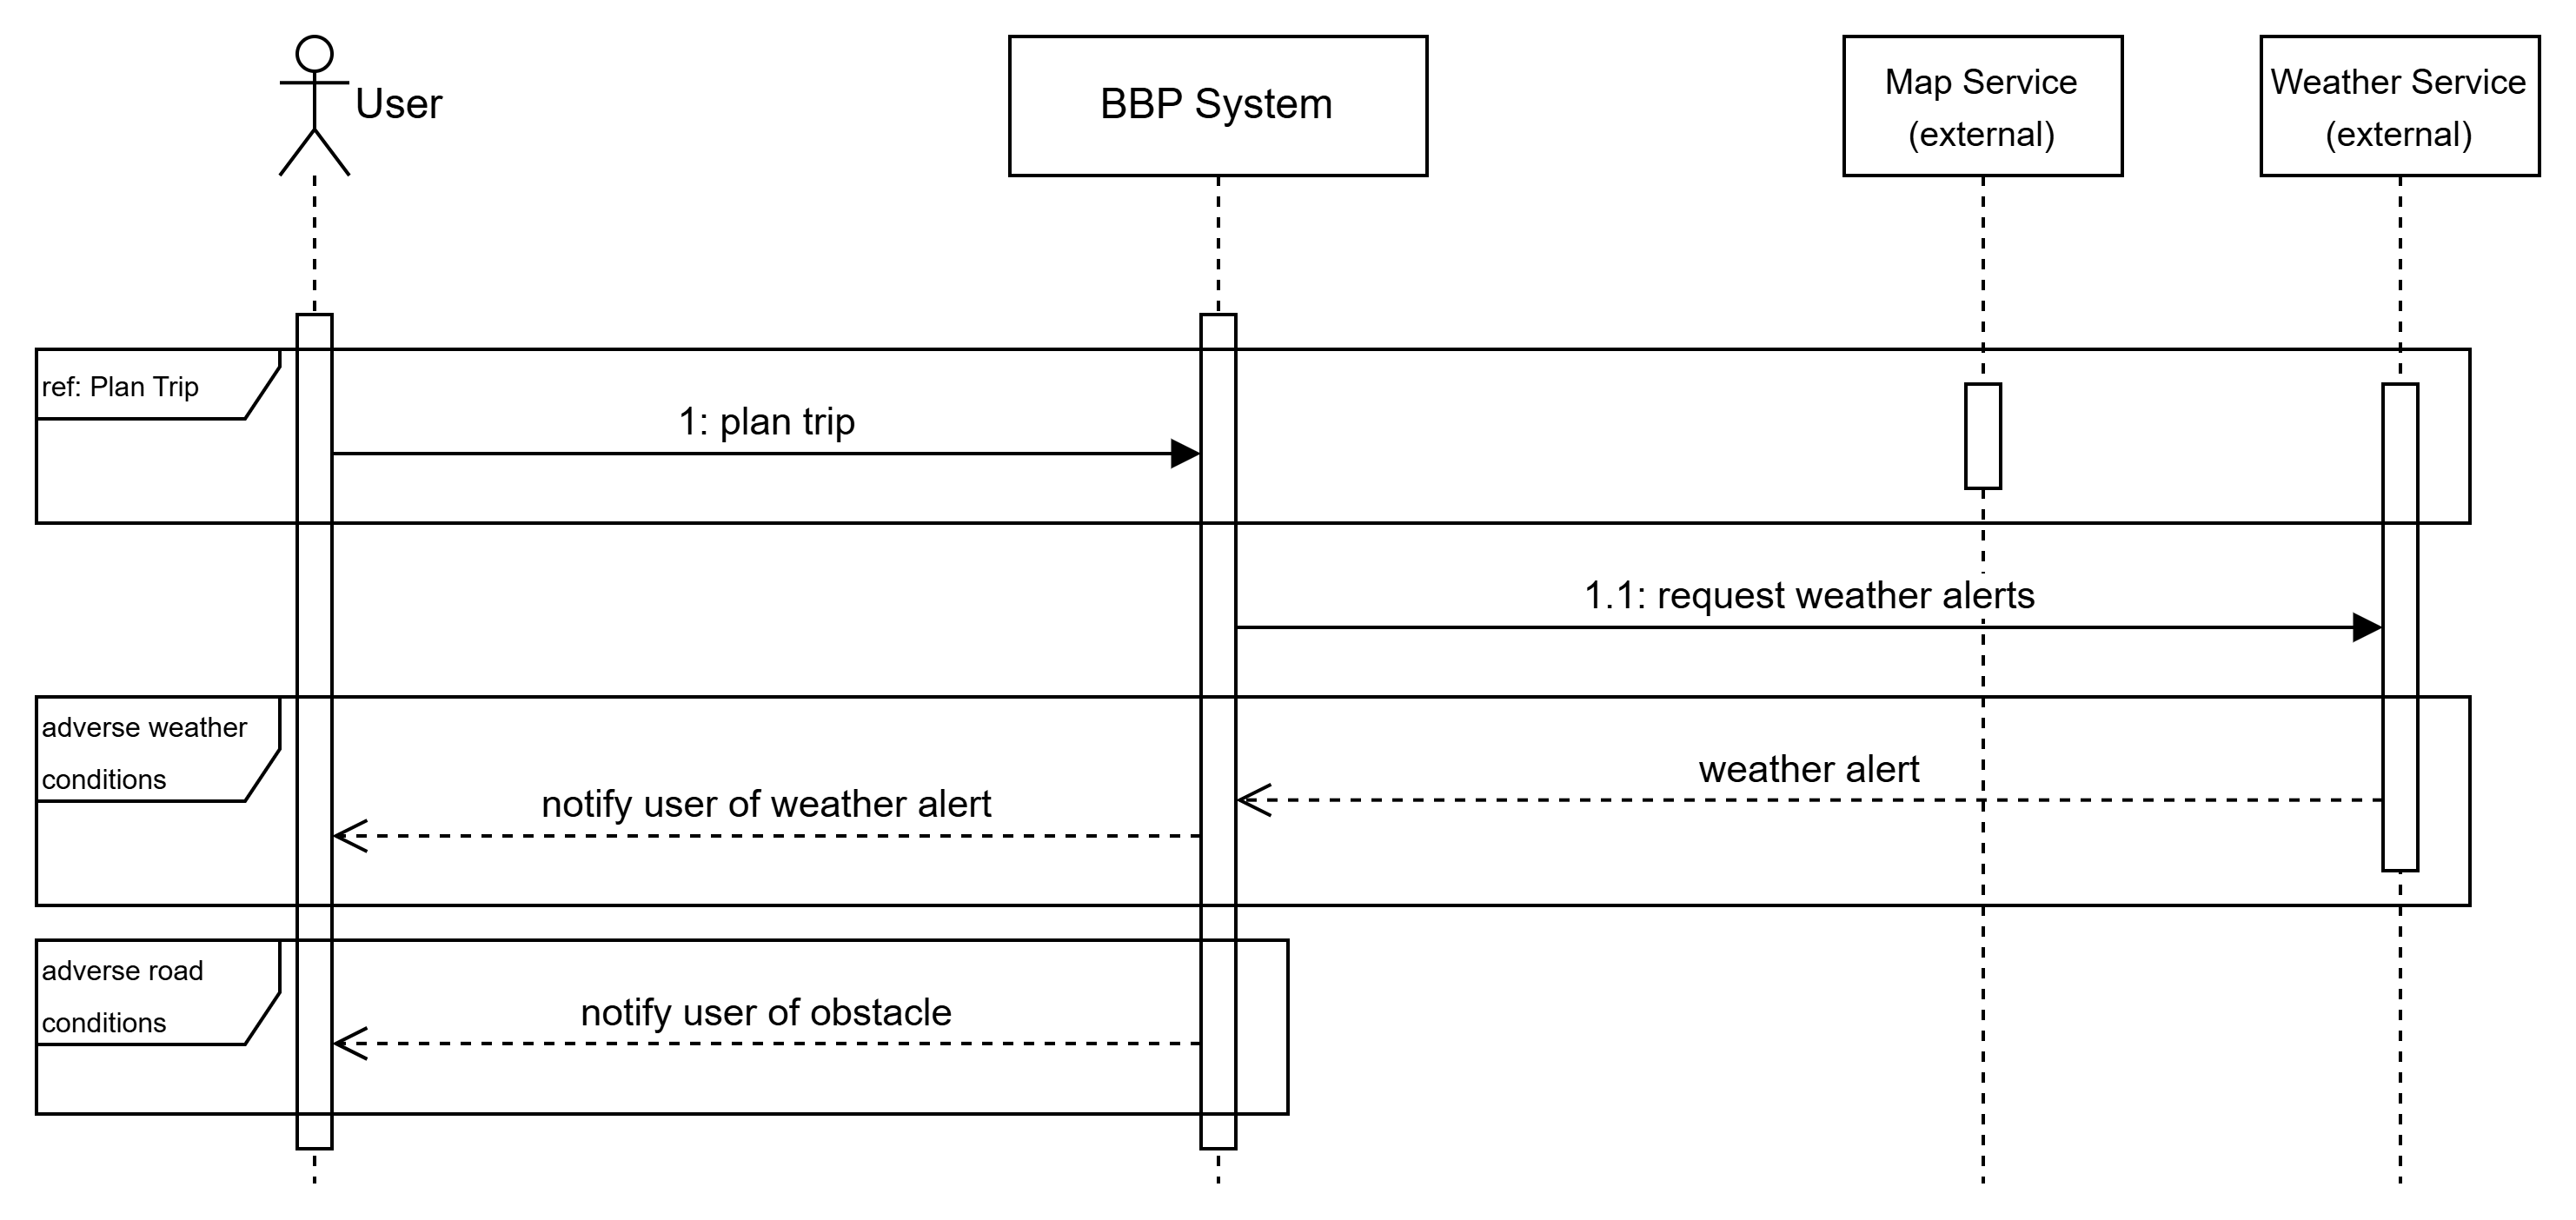
\includegraphics[width=0.9\linewidth]{RASD//source//images//diagrams/sd_trip_alert.png}
    \caption{Receive Trip Alerts Sequence Diagram.}
    \label{fig:sd_trip_alerts}
\end{figure}


\subsubsection{Mapping on Requirements}

\subsection{Performance Requirements}
The BBP system must ensure that the collected information is available both to registered and non-registered users. Also, the system performs well only if a large amount of registered users decide to publish the information about paths they went through during their biking sessions. That said, the system must support a large number of registered users, publishing a vast amount of data, and it must process all the queries from users concerning paths status and obstacles.
Given the considerable amount of users and data, the system must be able to easily scale-up while ensuring maximum performance. Another key aspect of BBP is availability: the system must ensure that the data is easily accessible to users and that the requested information is quickly available, all the time. Finally, the system must be capable of processing a large amount of data every time a user compiles a report of the biking trip he cycled.   

\subsection{Design Constraints}
\subsubsection{Standards Compliance}
\paragraph{Conformity Standards}
\begin{itemize}
    \item GDPR: The system manages users’ personal and administrative data, thus it must be compliant with the General Data Protection Regulation according to the European guidelines.
    \item ISO/IEC 27001 - Information Security Standard: The system must be characterized by a structured and comprehensive information security management, in order to protect sensitive information and be adaptable to new risks.
\end{itemize}

\paragraph{Development Standards}
\begin{itemize}
    \item ISO/IEC 12207: The system must be compliant to the software lifecycle management standard by applying the best practices in all its main processes.
\end{itemize}

\subsection{Software Constraints} \label{s: software_constraints}
Users access the BBP system via a mobile application, available both for Android and iOS, therefore the software constraints are relative to the mobile device used to access the platform:
\begin{itemize}
    \item For Android: the minimum supported version is Android 10 (API 29) for security reasons, as the application works with sensitive data, such as users' location and personal information.
    \item For iOS: the minimum supported version is iOS 16, according to average iOS requirements.
\end{itemize}

\subsubsection{Hardware Constraints}
Users access the BBP system via a mobile application, available both for Android and iOS, therefore the hardware constraints are relative to the mobile device used to access the platform:
\begin{itemize}
    \item The device used to access the platform must have a powerful enough processor in order to smoothly visualize GPU intensive data, such as maps. To this end, devices must have:
    \begin{itemize}
        \item Android: a quad-core ARMv7 or RM64 CPU architecture, with a clock speed of at least 1.5GHz, and an absolute minimum of 2GB of RAM. Also the device must support OpenGL ES 2.0 or higher, for rendering 3D graphics.
        \item iOS: at least an A12 Bionic processor and 3GB of RAM.
    \end{itemize}
    \item The device used to access the platform must have built-in sensors, such as gyroscope, accelerometer and GPS, in order to gather all the required information about the path and other metrics.
    \item The device used to access the platform must have a stable internet connection, so the user can retrieve his personal activities, planned trips and statistics. Also an internet connection is crucial for searching routes between the departure and destination points, and the status of each street. Furthermore, the internet connection is necessary to retrieve community shared obstacles and add new obstacles in the report review phase.
\end{itemize}

\subsection{Software System Attributes}
\subsubsection{Reliability}
The BBP system must preserve a large amount of data retrieved from registered users, thus it should replicate data and ensure its consistency across multiple nodes. Despite the higher financial cost, this solution prevents data loss and enables data recovery. Also, the system periodically runs checksum verification in order to validate stored data against possible corruptions. Furthermore, the system must have a secure multi-factor authentication backdoor access for administrators only, in order to ensure emergency maintenance. Note that, the usage of the backdoor must be monitored and every action reported into a log, so maximum security is guaranteed.

\subsubsection{Availability}
The BBP system must guarantee a highly available service, quickly accessible through users' mobile devices. The design of the system must ensure 99.9\% (3-nines) of uptime, allowing only a maximum of 9 hours of downtime a year. As already said in the previous section, the system should be partitioned into multiple nodes, to ensure reliability as well as redundancy of the data. In case of node failure, the system must automatically detect it and redirect traffic to running healthy replicas, in order to maintain service continuity. This partition also allows geographical redundancy, for data replication across different physical regions to protect it against localized data centre outages. Finally, the system must implement circuit breakers between components into its design to prevent cascading failures.

\subsubsection{Security}
The BBP system allows users to sign in and sign up to the platform via email and password. This represents a highly sensitive part of the system, requiring some extra considerations. The password is salted, peppered and hashed with advanced encryption algorithms like \textit{Argon2id}. The salt is randomly generated for every user at registration, then hashed and stored in the database with the encrypted password. The pepper is the same for all users and stored in a secure storage on the users' device. In order to transfer the hashed password and the hashed salt to the back-end in a secure manner, the data is encrypted and transmitted via HTTPS using the TLS 1.3 protocol. Also, the report data sent to the server and the client requested information must be transferred via the HTTPS protocol, to ensure security and consistency.  

\subsubsection{Maintainability}
The client side of the BBP system consists of a mobile application, so maintainability is crucial. To ensure this software attribute, the mobile application is designed using the Model-View-ViewModel (MVVM) pattern, which makes it easier to separate the UI layer, from the business logic and data layer. Also, the MVVM pattern ensures Unidirectional Data Flow (UDF), decoupling the components that display state in the UI, from the ones that store and modify the state. Also, the application is subdivided into modules, so it is optimized for scalability and maintainability. All the code must be well documented and tested, to maintain a high quality standard.

The server side of the BBP system must be highly modular and ideally adopt a micro-service architecture, so it is more maintainable, testable and scalable. Every component of the server must have a clearly defined API, so it is easier for developers to integrate new components into the system.

\subsubsection{Portability}
The client side of the BBP system consists of a mobile application, from which users can access the platform. For this reason, the application is compatible with both Android and iOS operating systems (as specified in \ref{s: software_constraints}). The application UI must adapt to different aspect ratios, resolutions and orientations, and also different screen sizes, ranging from 4.7 inches to 12.9 inches. All the users' data is stored and synchronized in the back-end, so it's possible for users to switch from one device to another with ease. Also, users can request to export their data in a standard JSON format so they can move it to a different service.